\section{Appendix}

\begin{figure}[h!]
%\hspace{-2.0cm}
\center
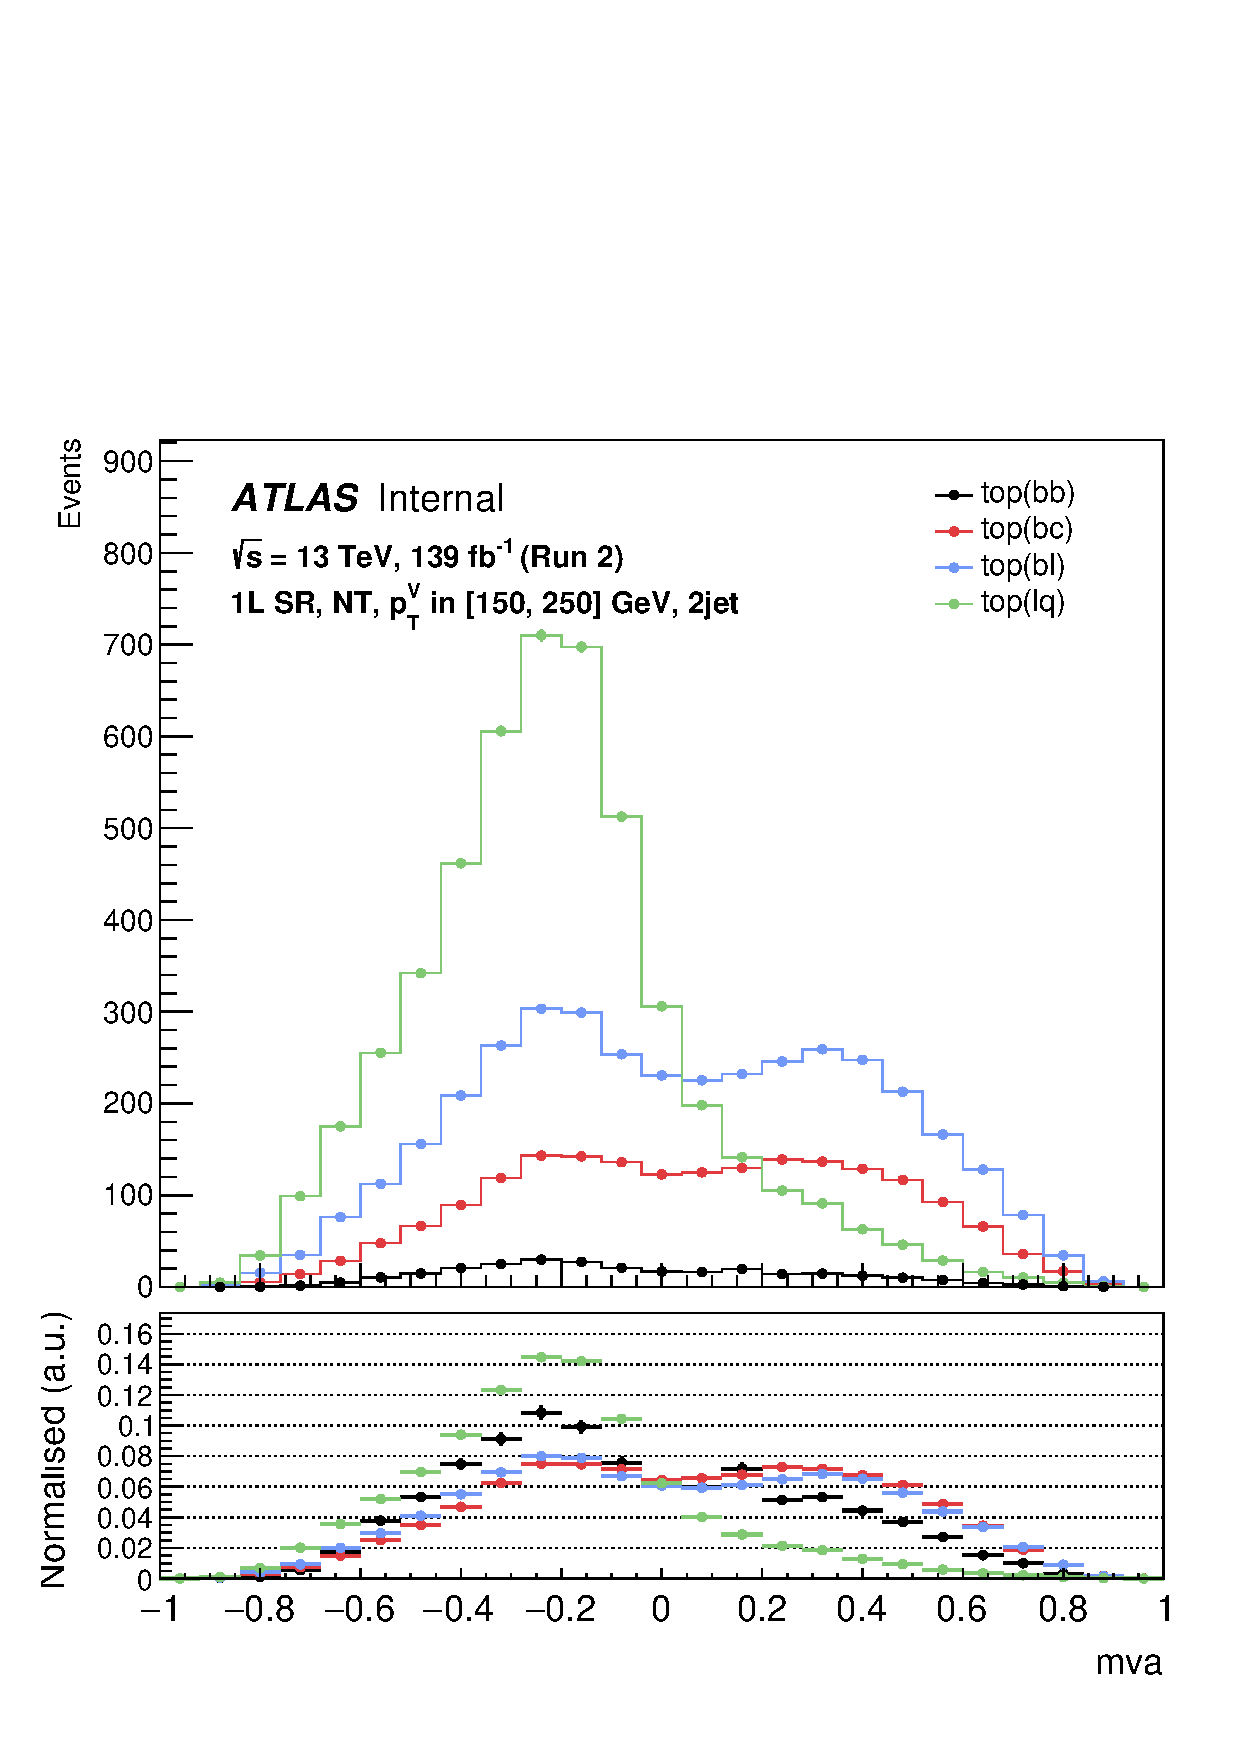
\includegraphics[scale=0.253]{Images/VH/top/OneLepton_top_1nttag2jet_SR_150_250ptv_mva.pdf}
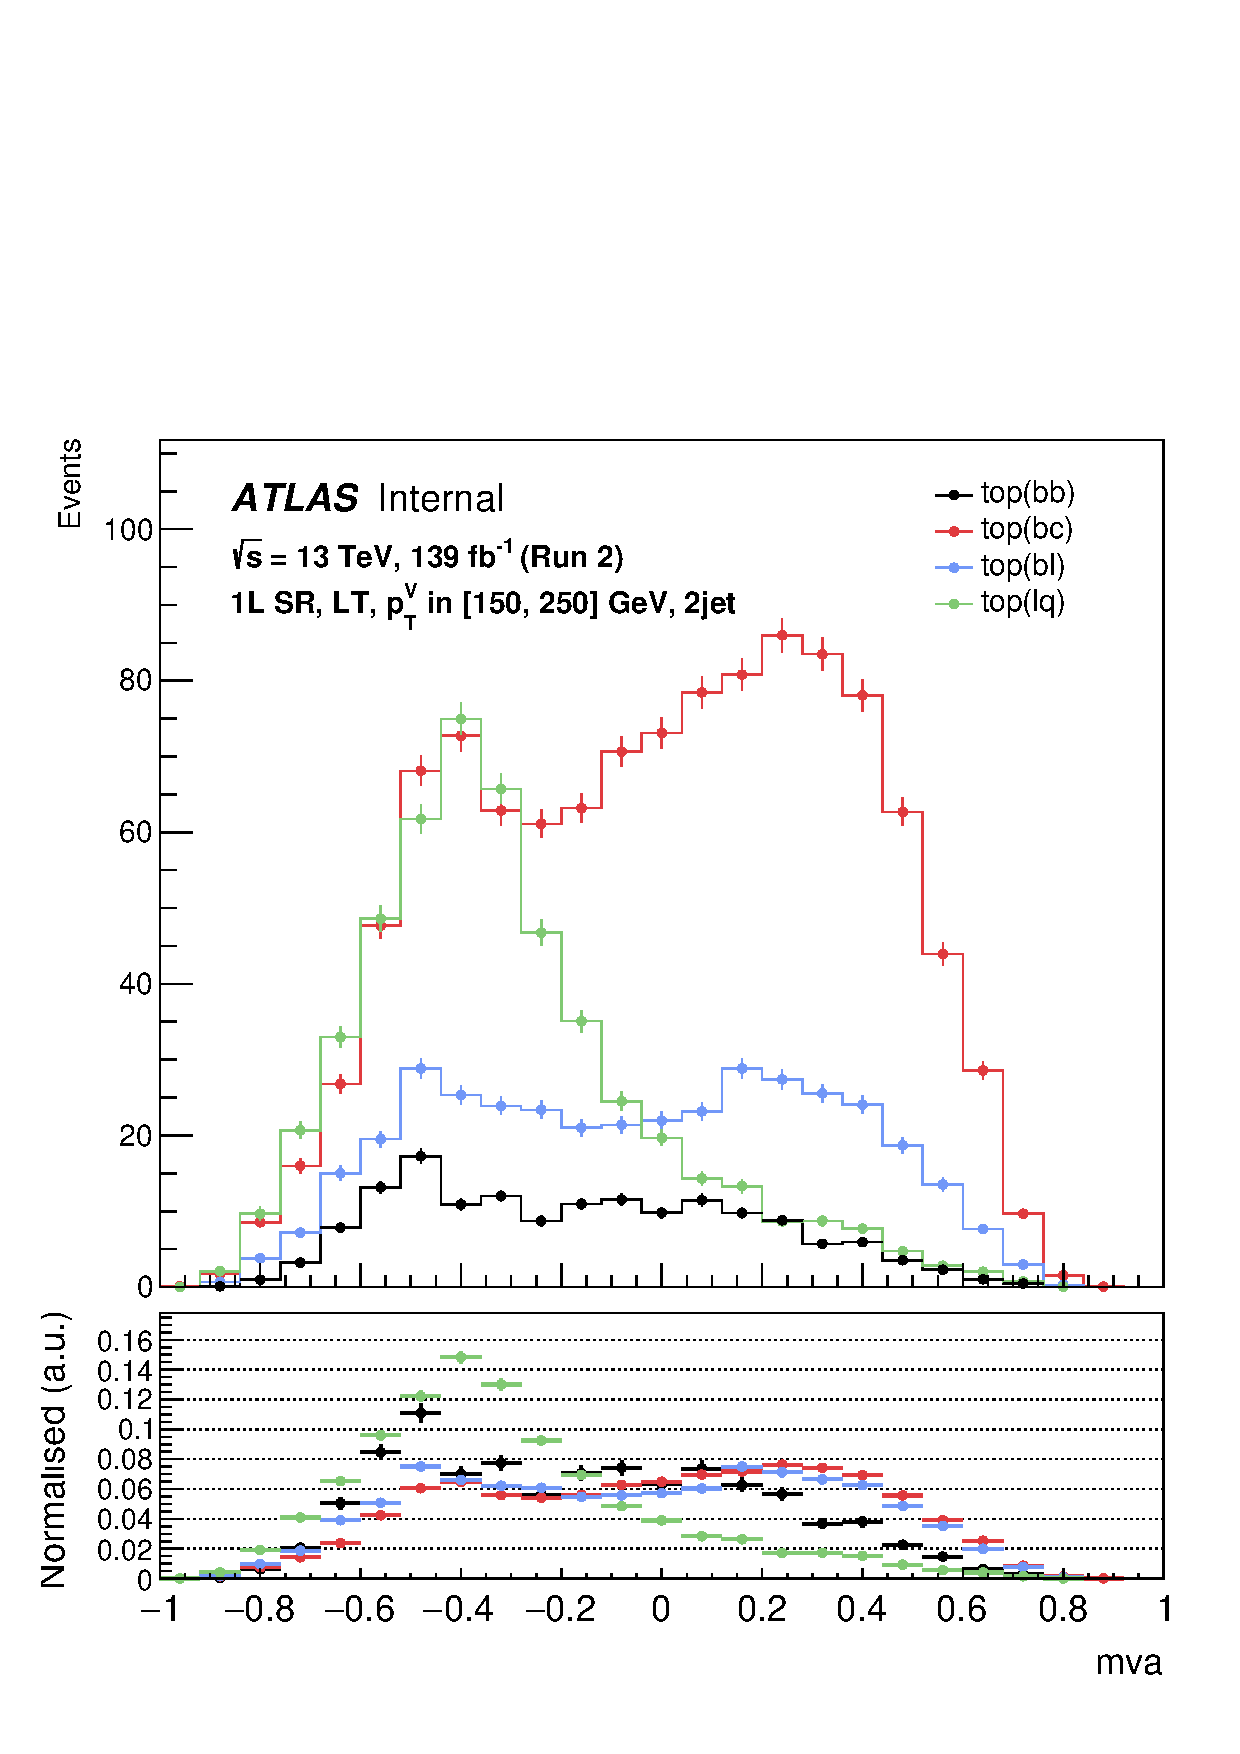
\includegraphics[scale=0.253]{Images/VH/top/OneLepton_top_2lttag2jet_SR_150_250ptv_mva.pdf}
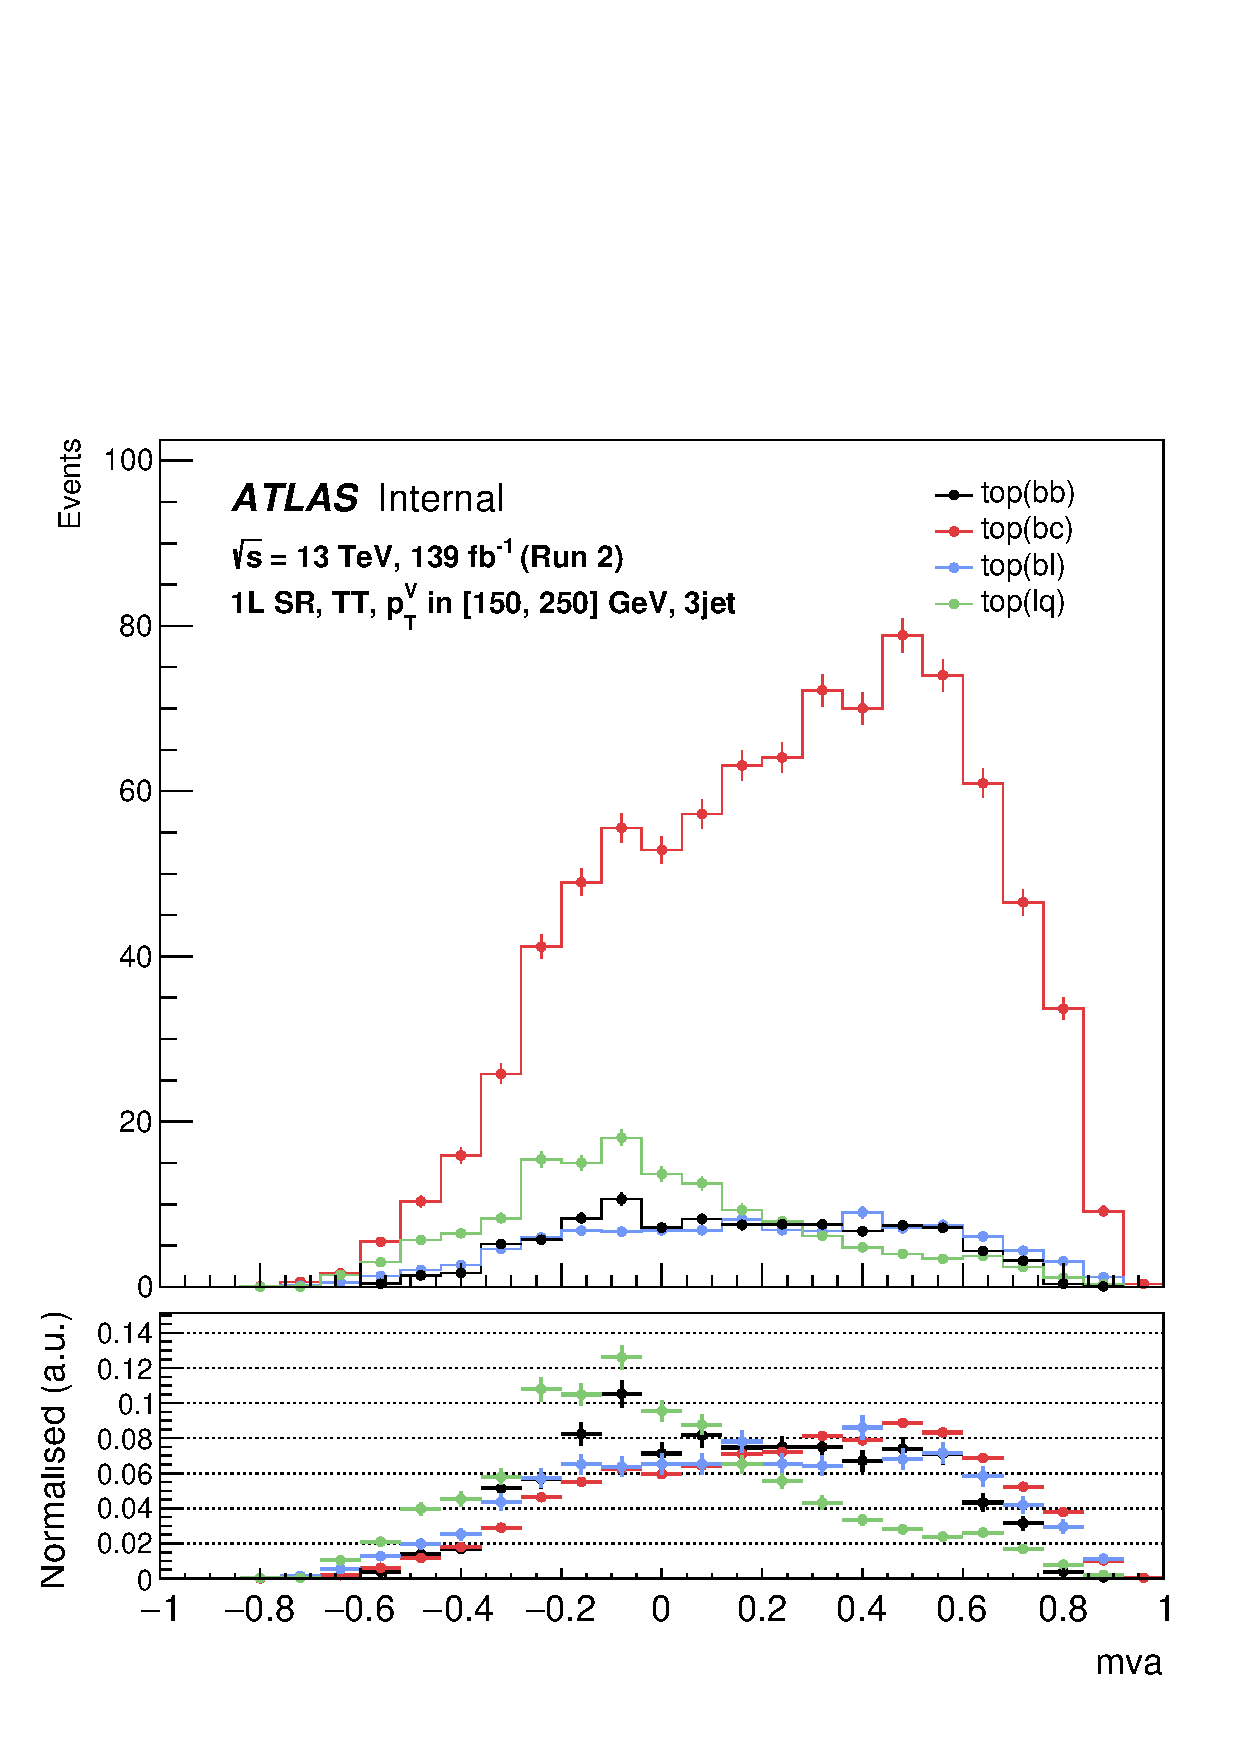
\includegraphics[scale=0.253]{Images/VH/top/OneLepton_top_2tttag3jet_SR_150_250ptv_mva.pdf} \\

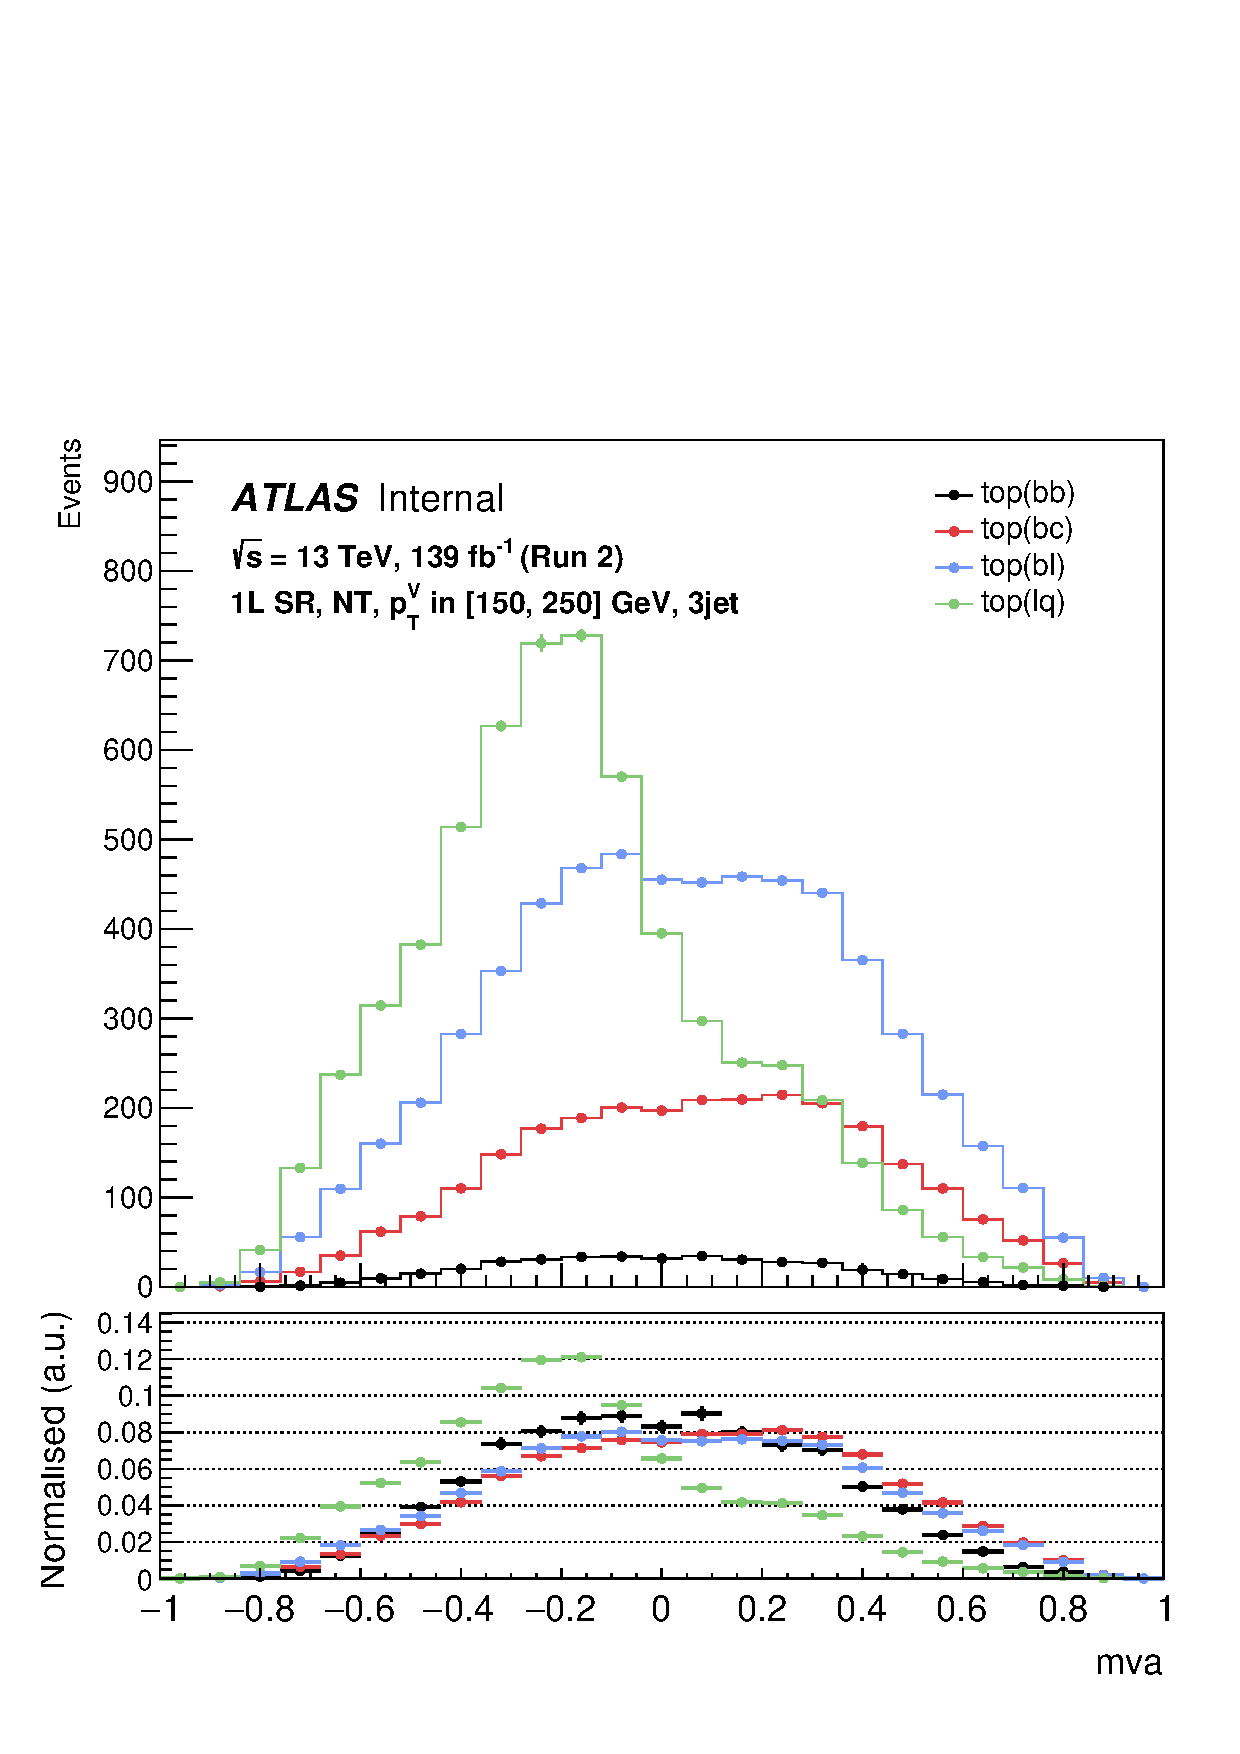
\includegraphics[scale=0.253]{Images/VH/top/OneLepton_top_1nttag3jet_SR_150_250ptv_mva.pdf}
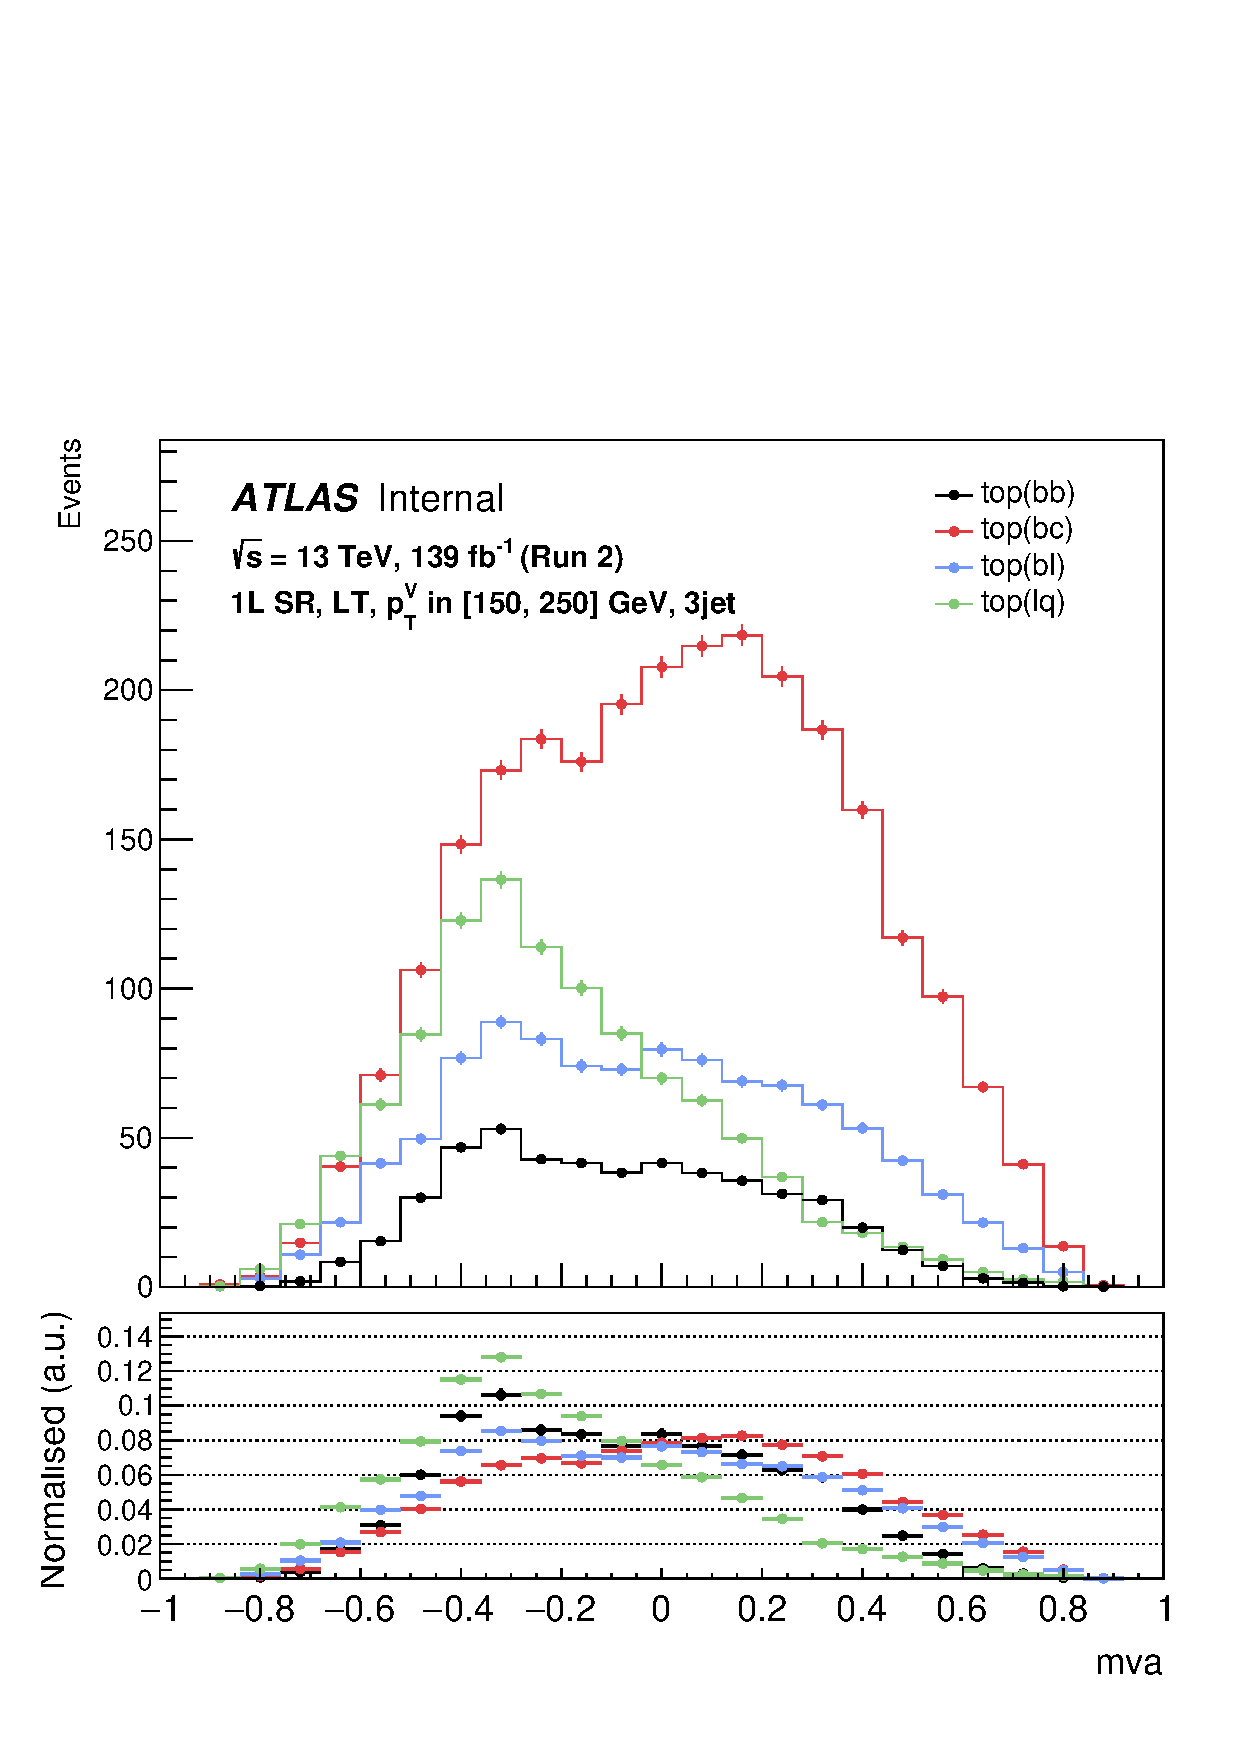
\includegraphics[scale=0.253]{Images/VH/top/OneLepton_top_2lttag3jet_SR_150_250ptv_mva.pdf}
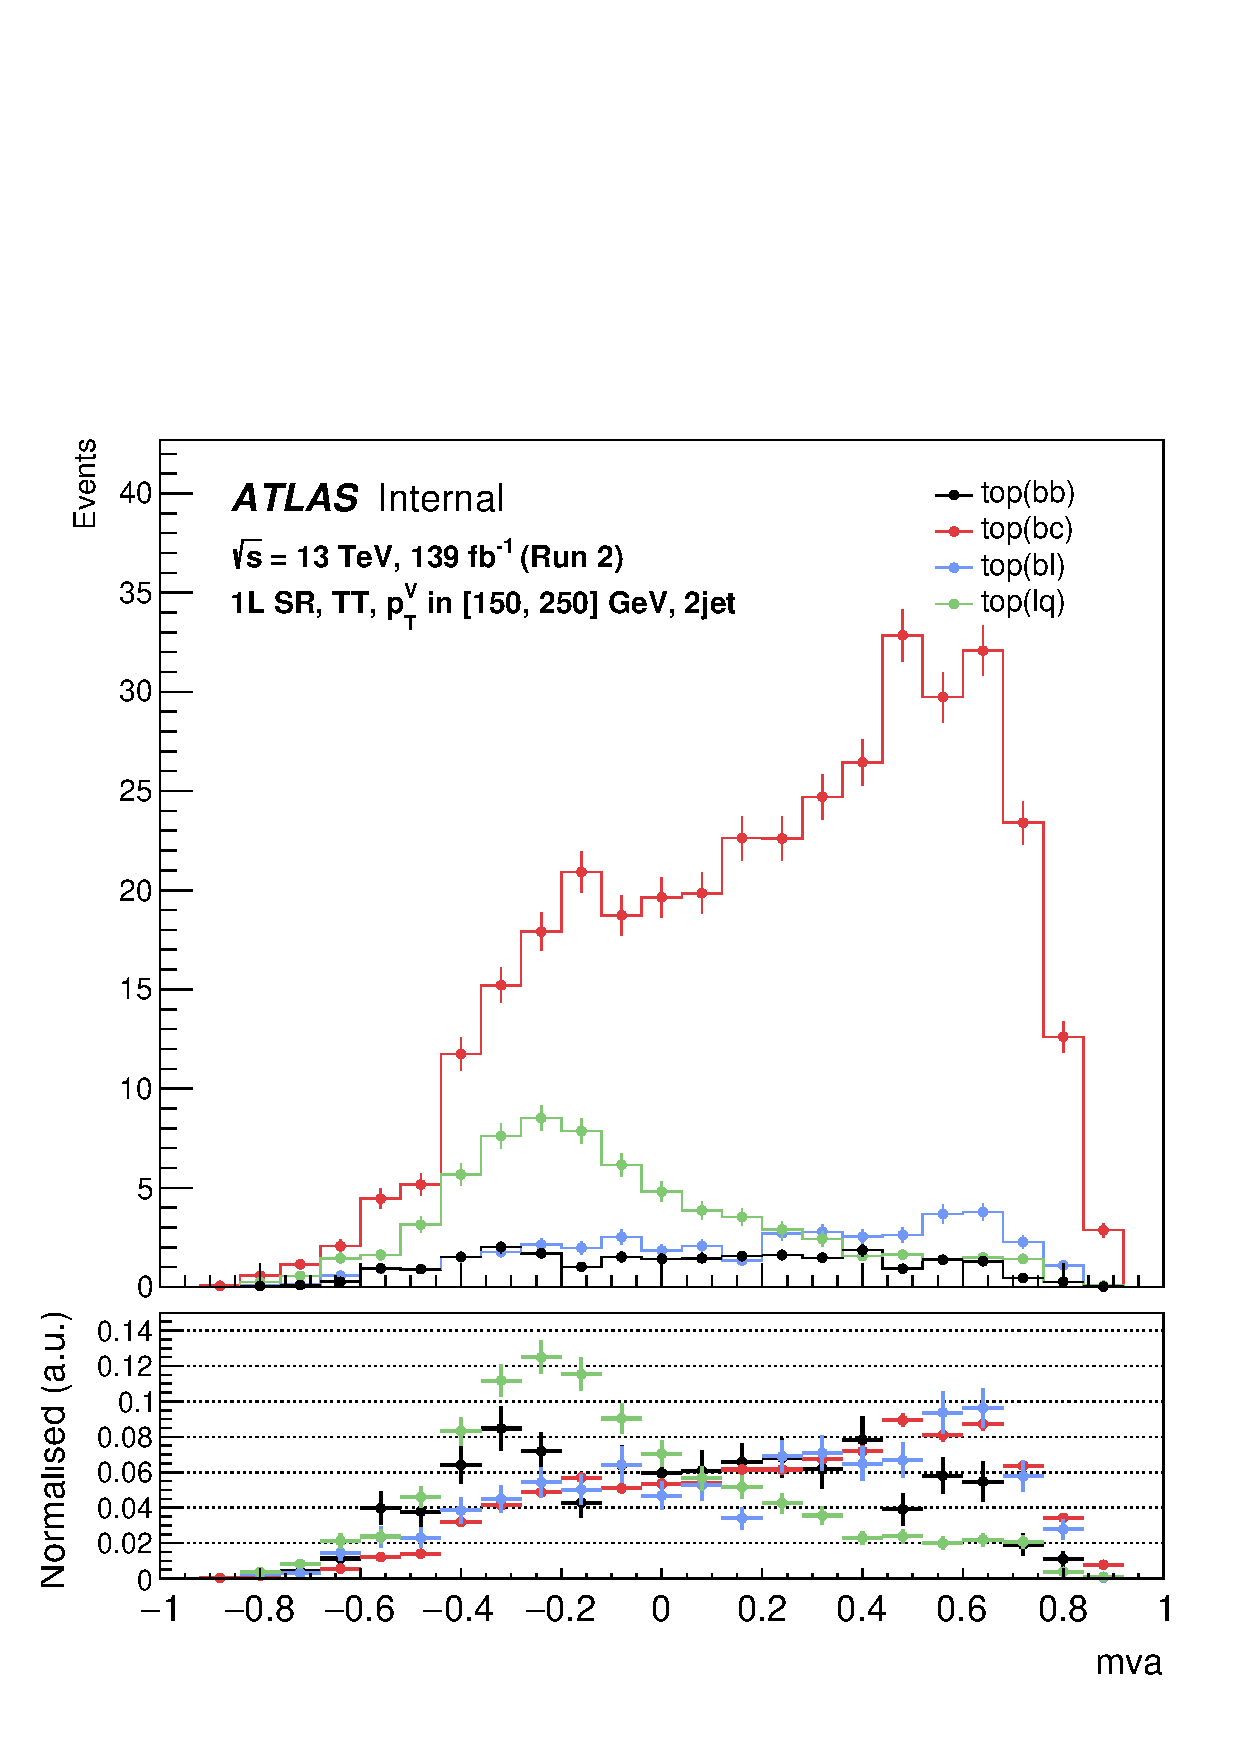
\includegraphics[scale=0.253]{Images/VH/top/OneLepton_top_2tttag2jet_SR_150_250ptv_mva.pdf}
\caption{The top components in the 1L signal regions BDT distributions in the low [150-250] $p_T^V$ range. NT: left; LT: centre; TT: right. Top: 2 jets, bottom: 3 jets.} 
\label{fig:topSRslowptv}
\end{figure}


\begin{figure}[h!]
%\hspace{-2.0cm}
\center
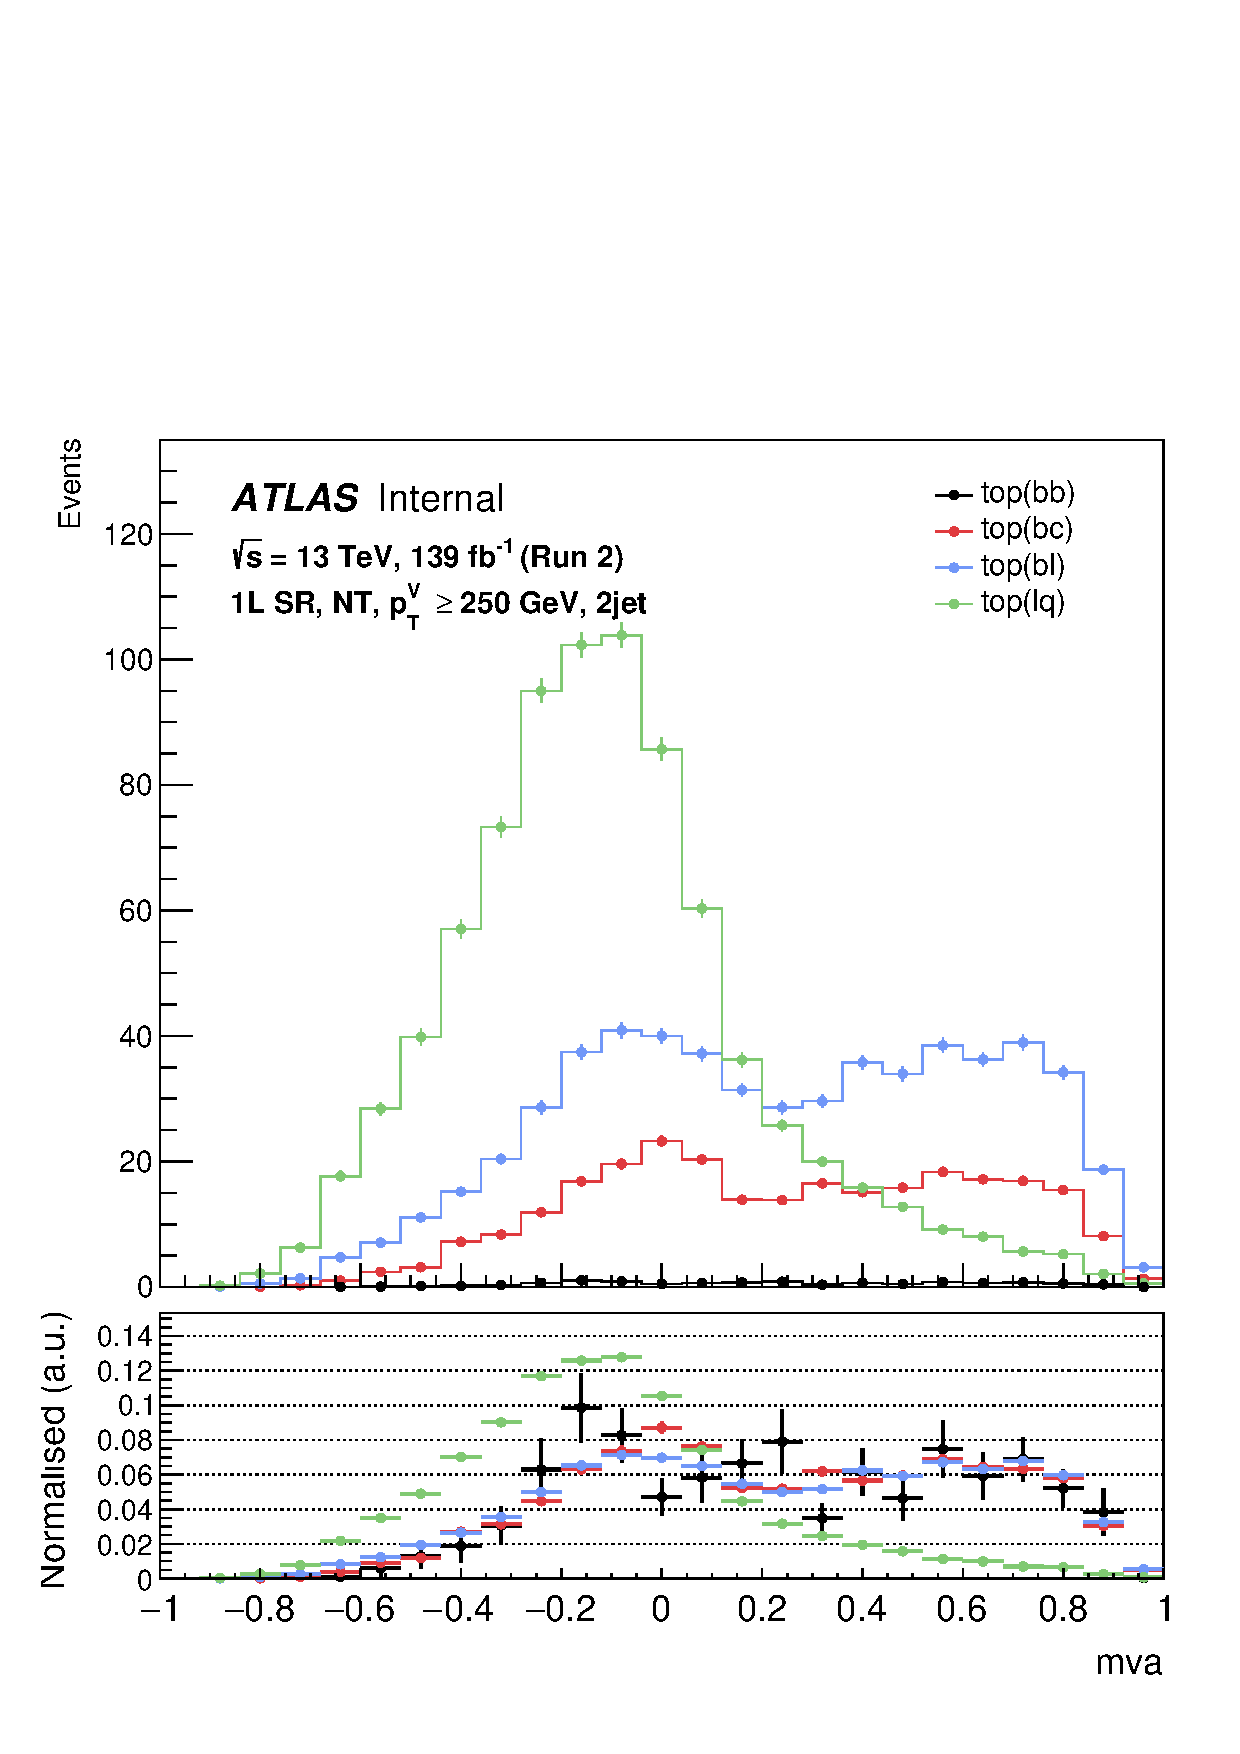
\includegraphics[scale=0.253]{Images/VH/top/OneLepton_top_1nttag2jet_SR_250ptv_mva.pdf}
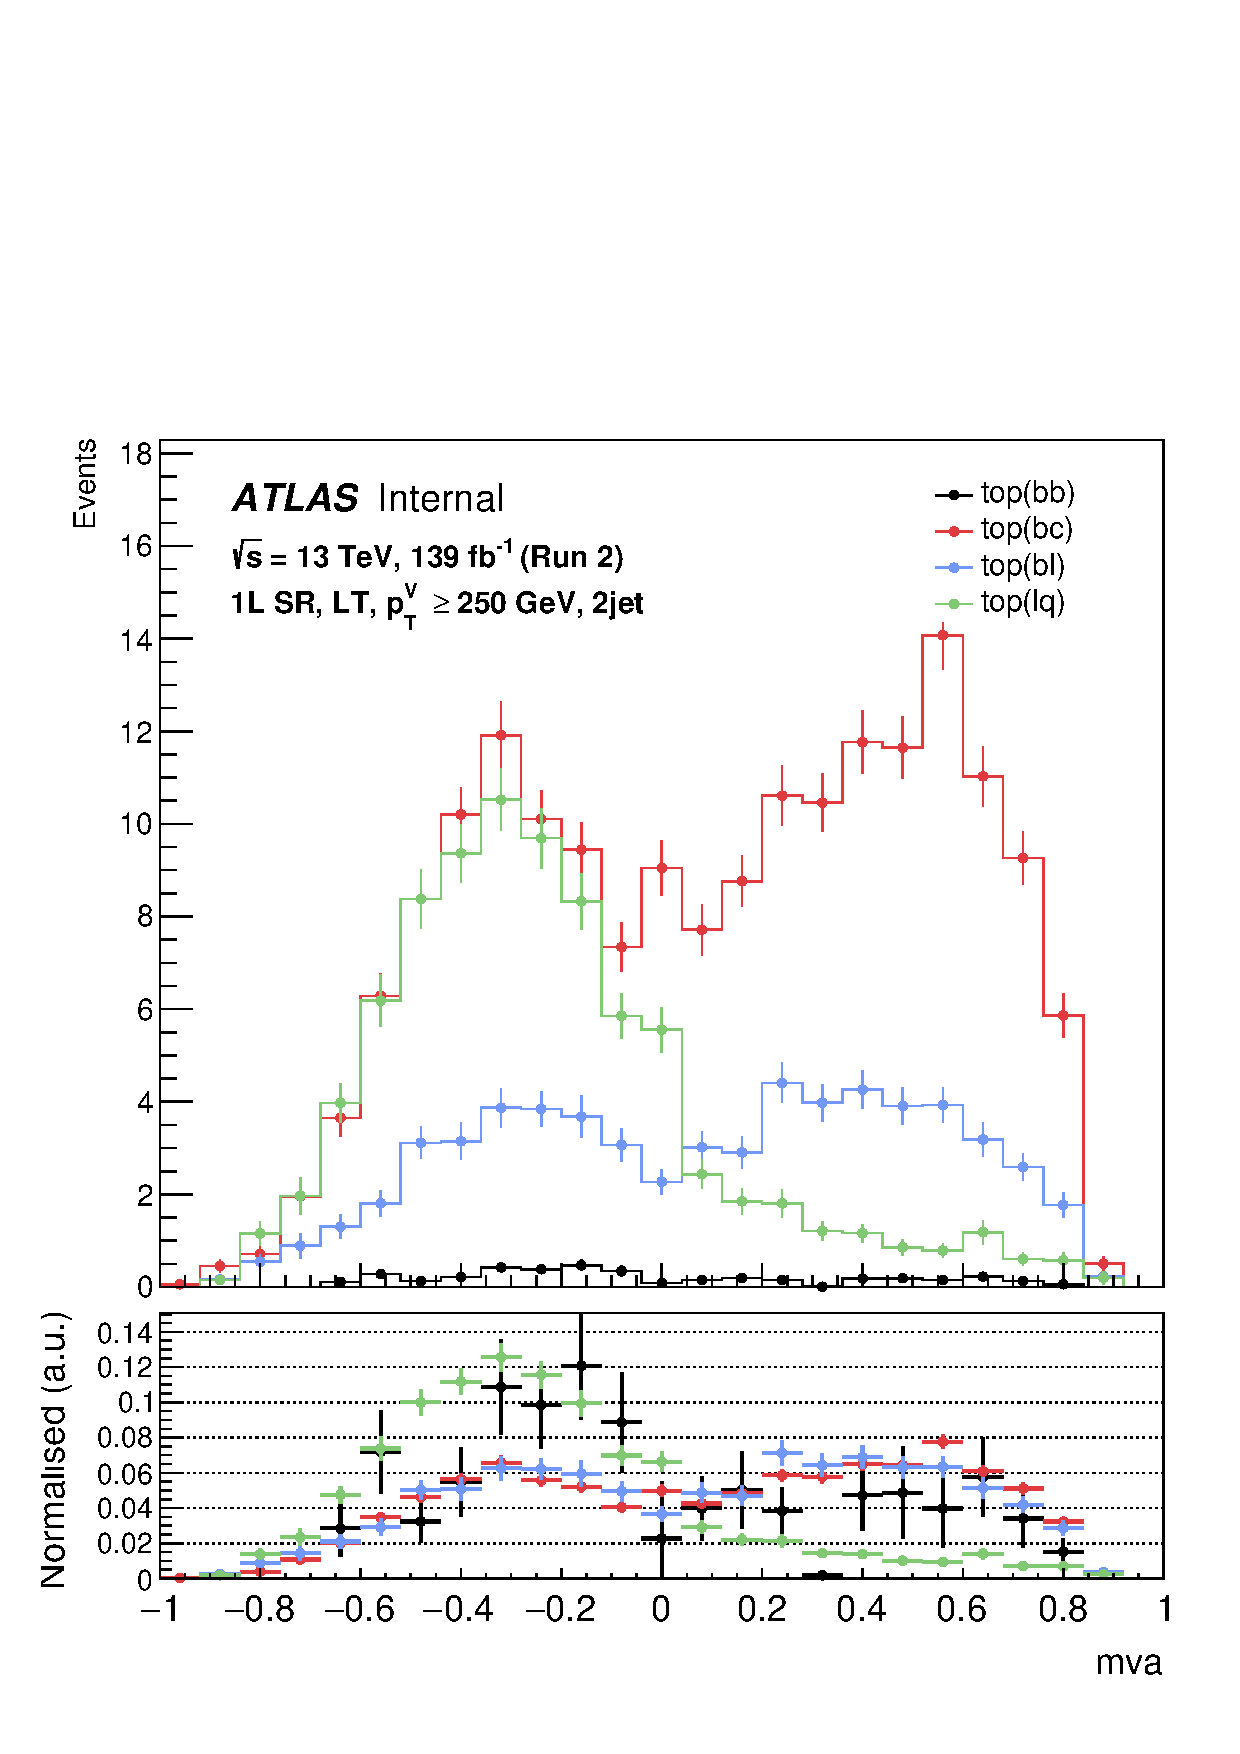
\includegraphics[scale=0.253]{Images/VH/top/OneLepton_top_2lttag2jet_SR_250ptv_mva.pdf}
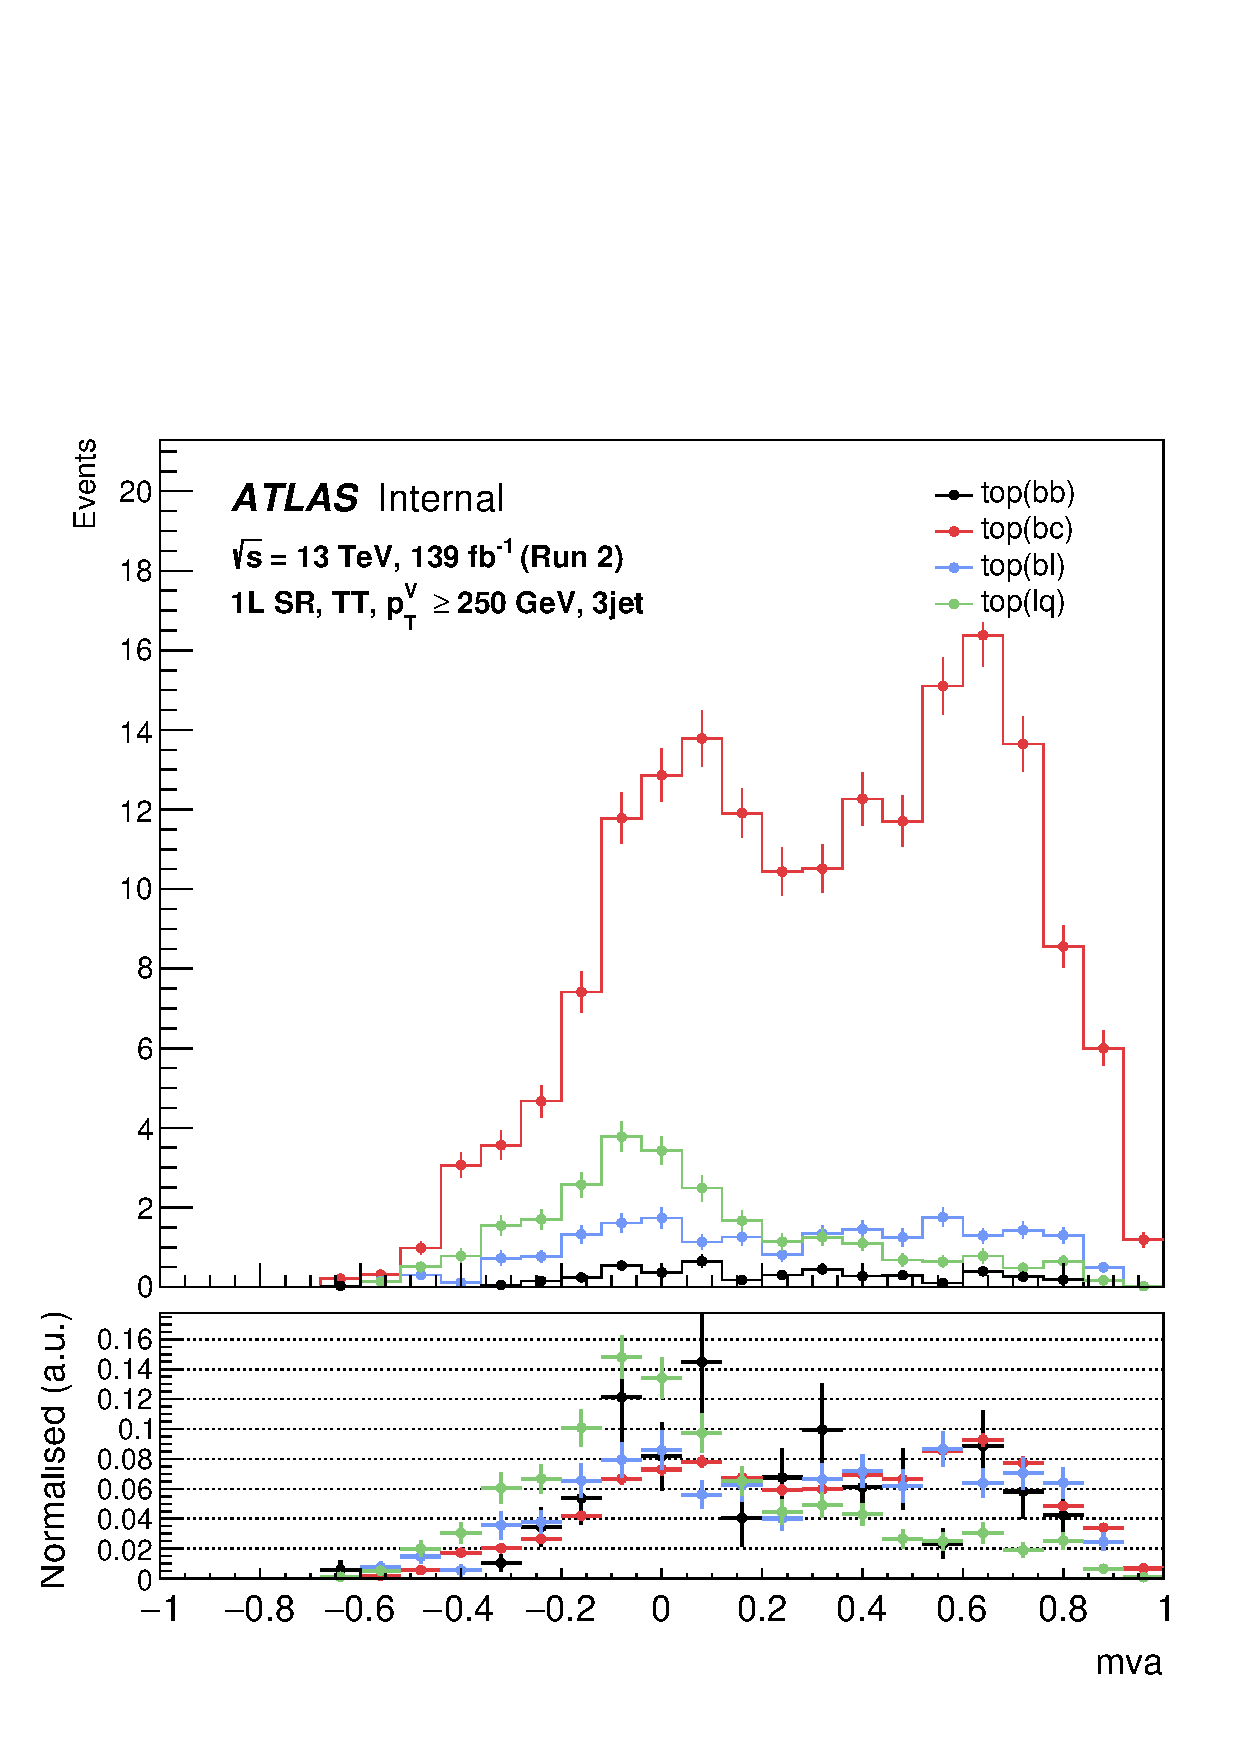
\includegraphics[scale=0.253]{Images/VH/top/OneLepton_top_2tttag3jet_SR_250ptv_mva.pdf} \\

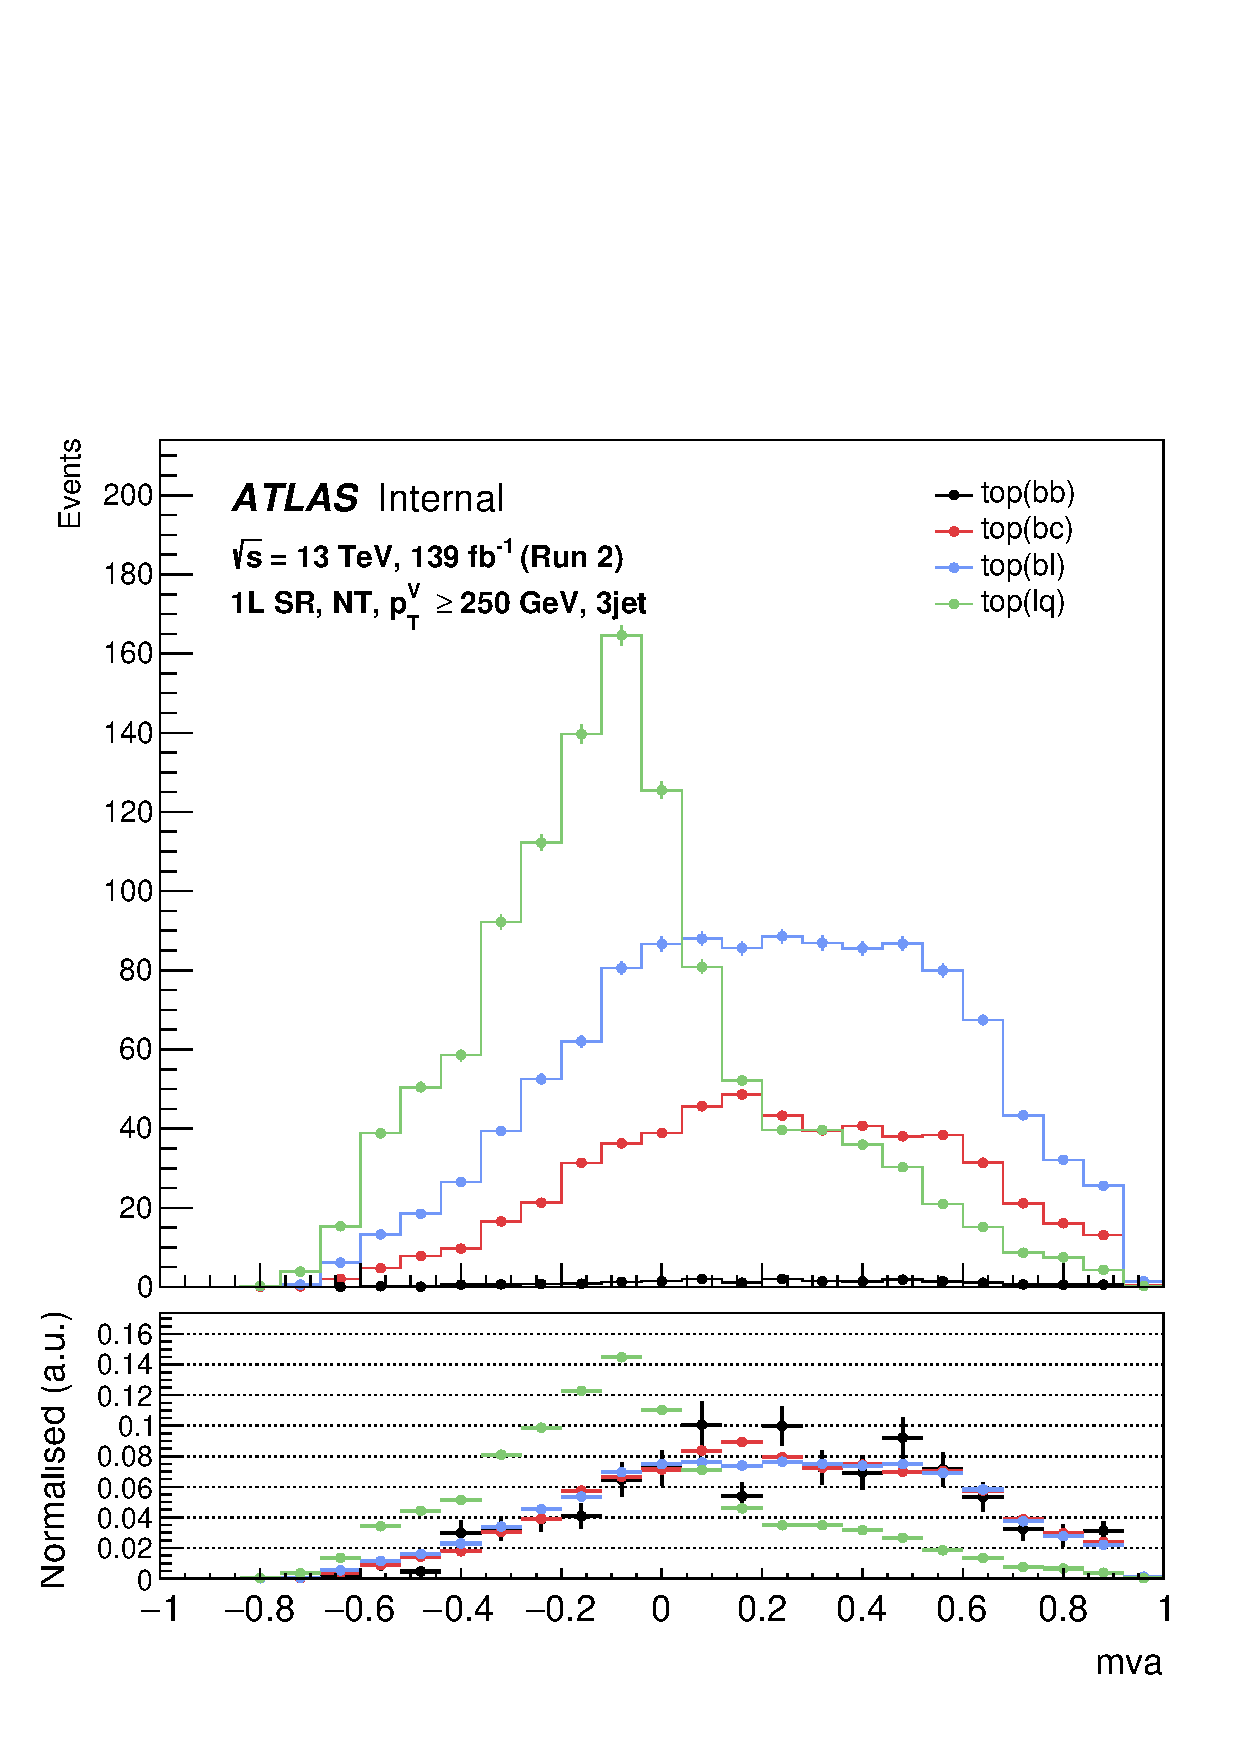
\includegraphics[scale=0.253]{Images/VH/top/OneLepton_top_1nttag3jet_SR_250ptv_mva.pdf}
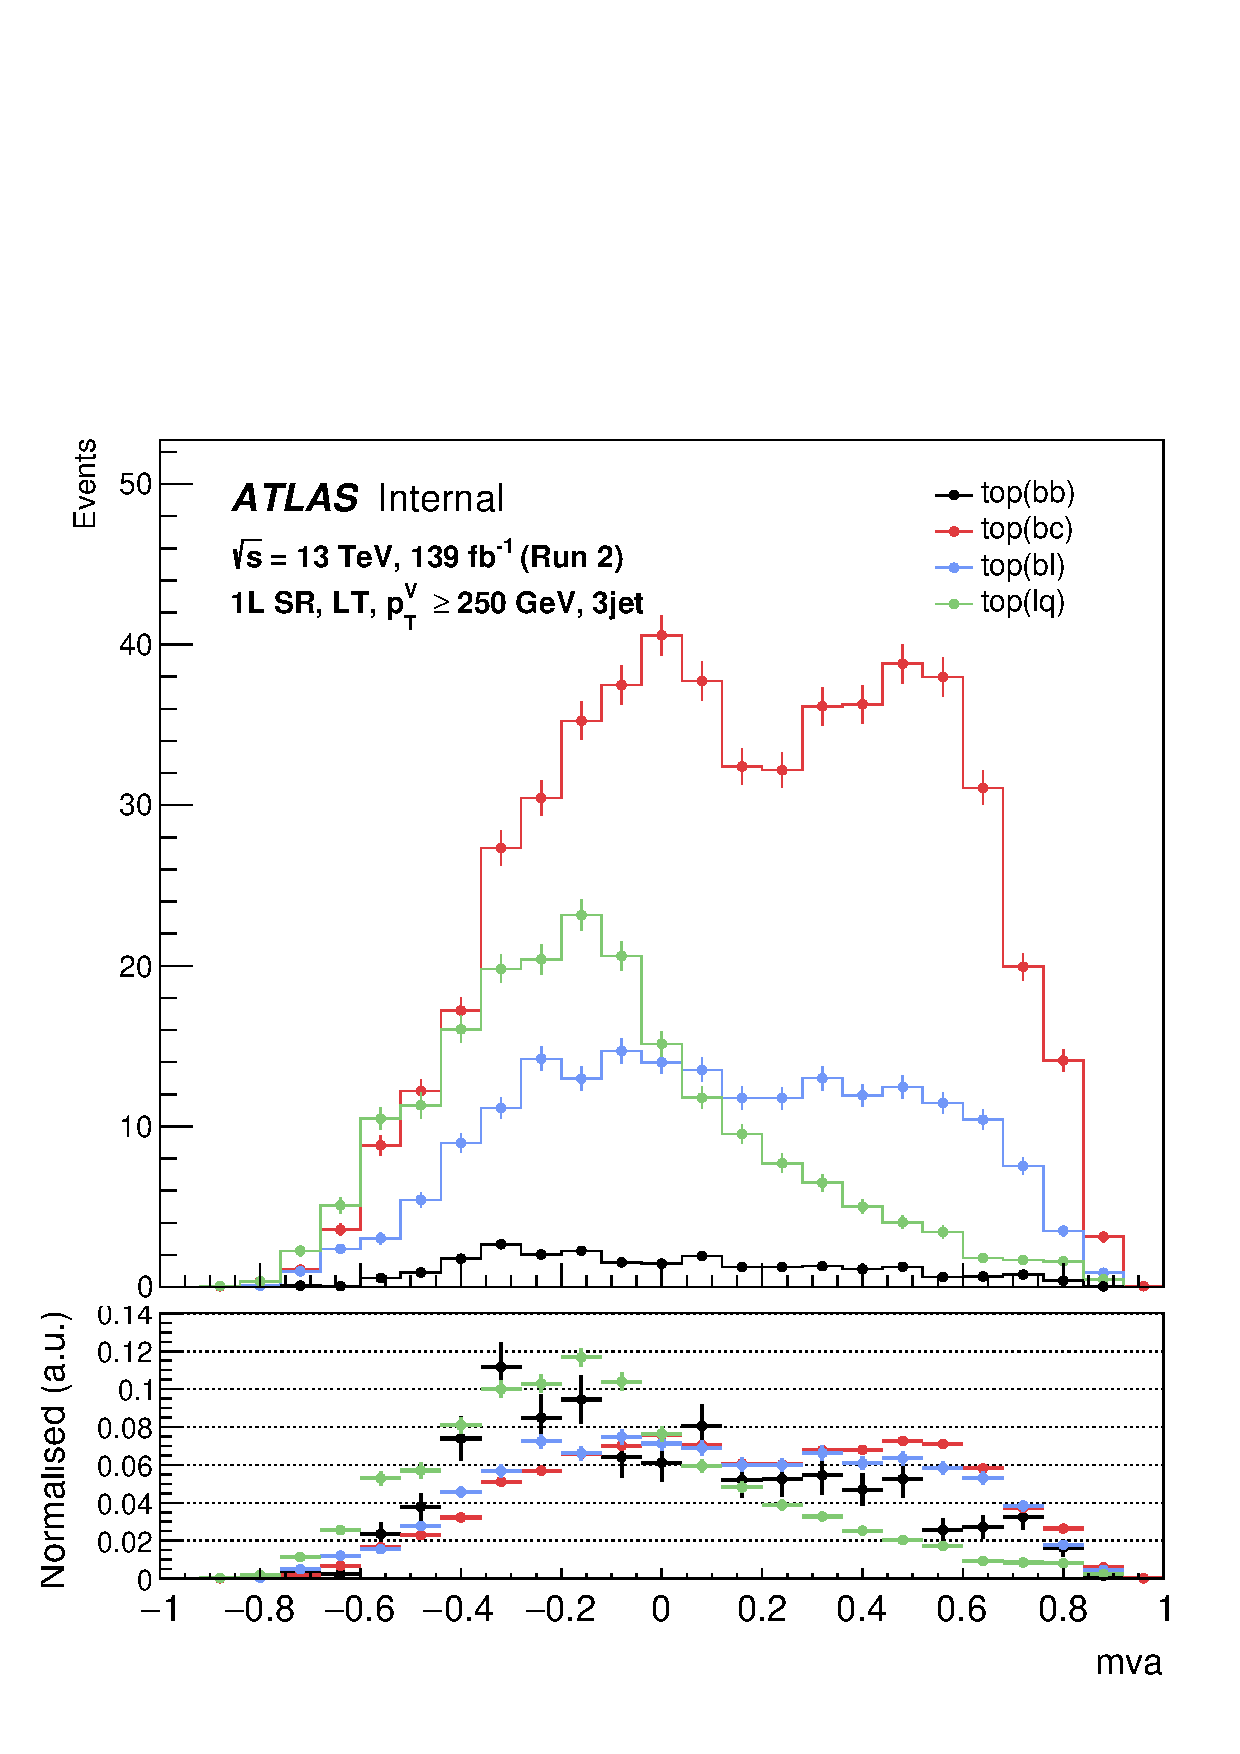
\includegraphics[scale=0.253]{Images/VH/top/OneLepton_top_2lttag3jet_SR_250ptv_mva.pdf}
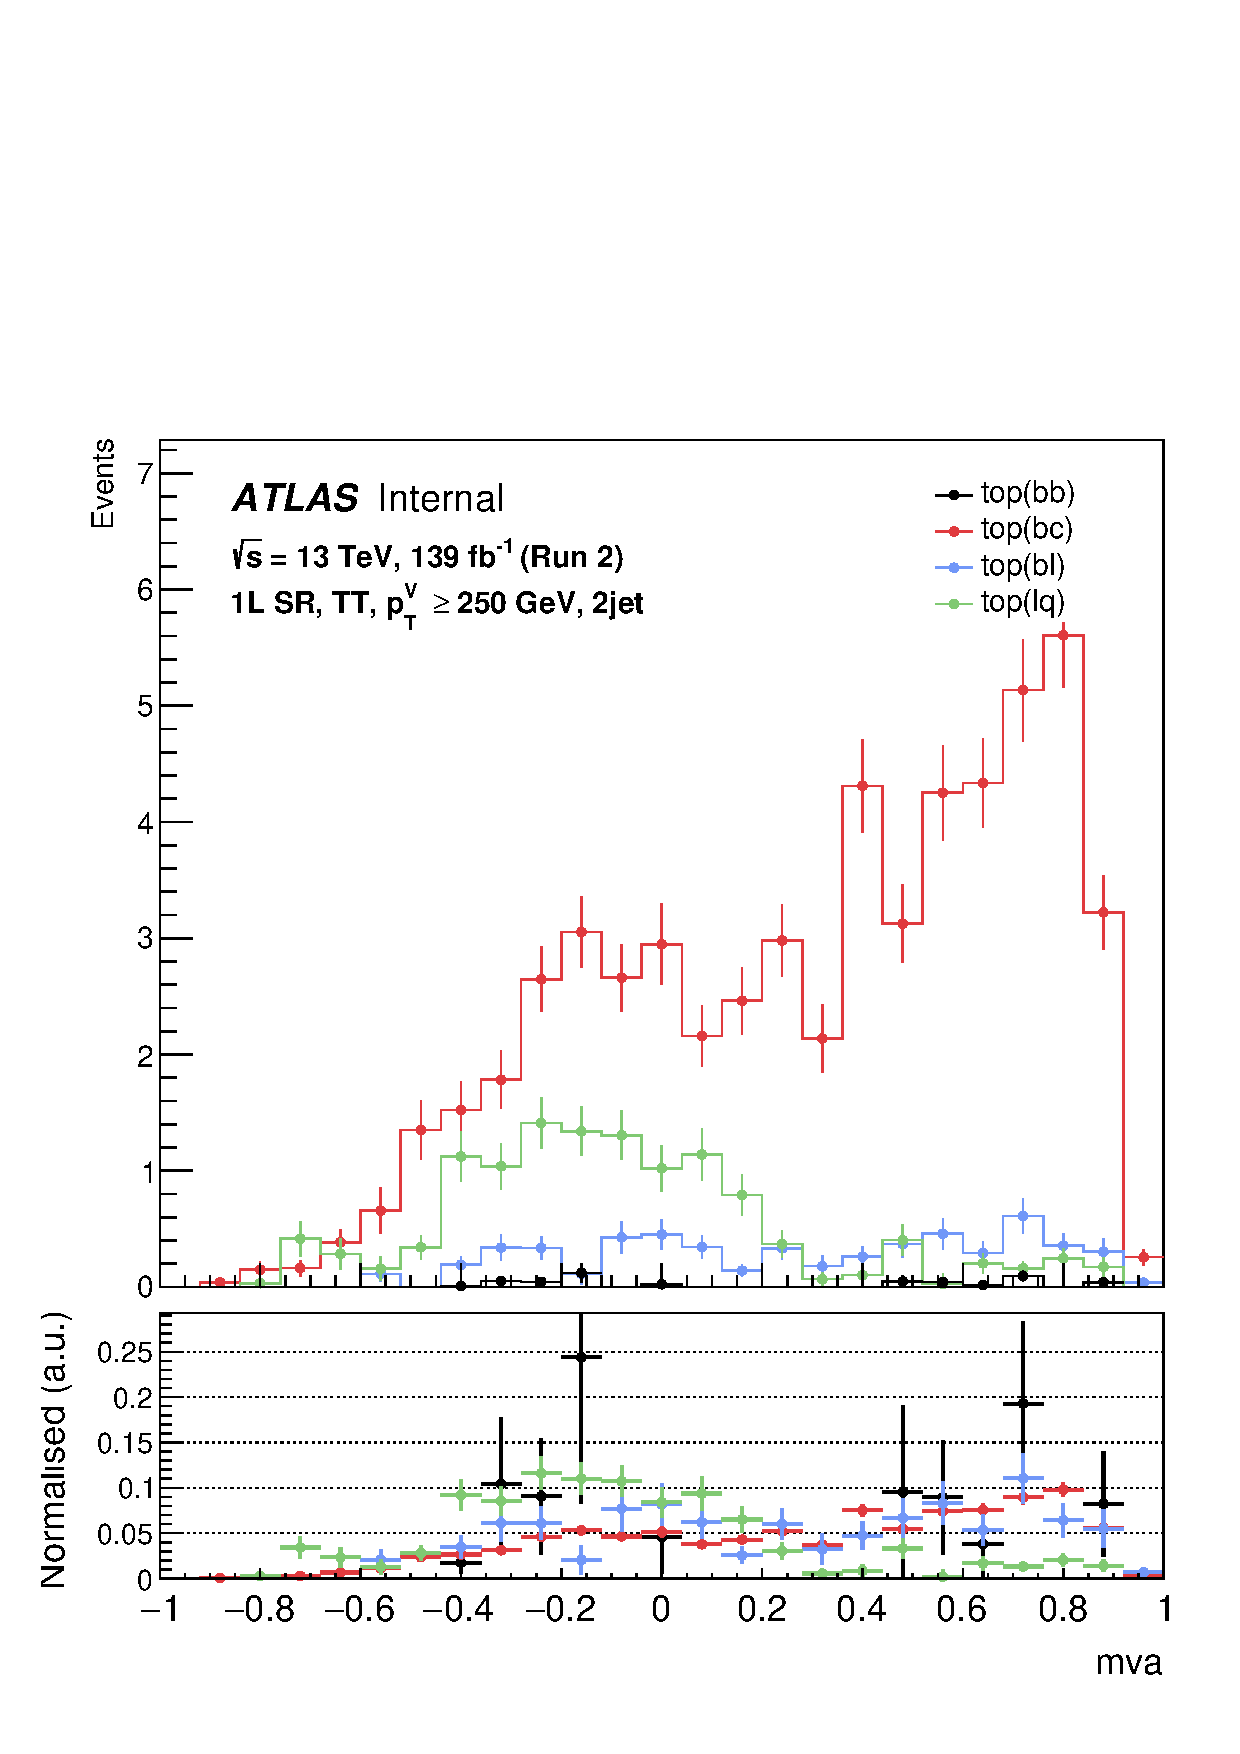
\includegraphics[scale=0.253]{Images/VH/top/OneLepton_top_2tttag2jet_SR_250ptv_mva.pdf}
\caption{The top components in the 1L signal regions BDT distributions in the high > 250 $p_T^V$ range. NT: left; LT: centre; TT: right. Top: 2 jets, bottom: 3 jets.} 
\label{fig:topSRshighptv}
\end{figure}

\begin{figure}[h!]
%\hspace{-2.0cm}
\center
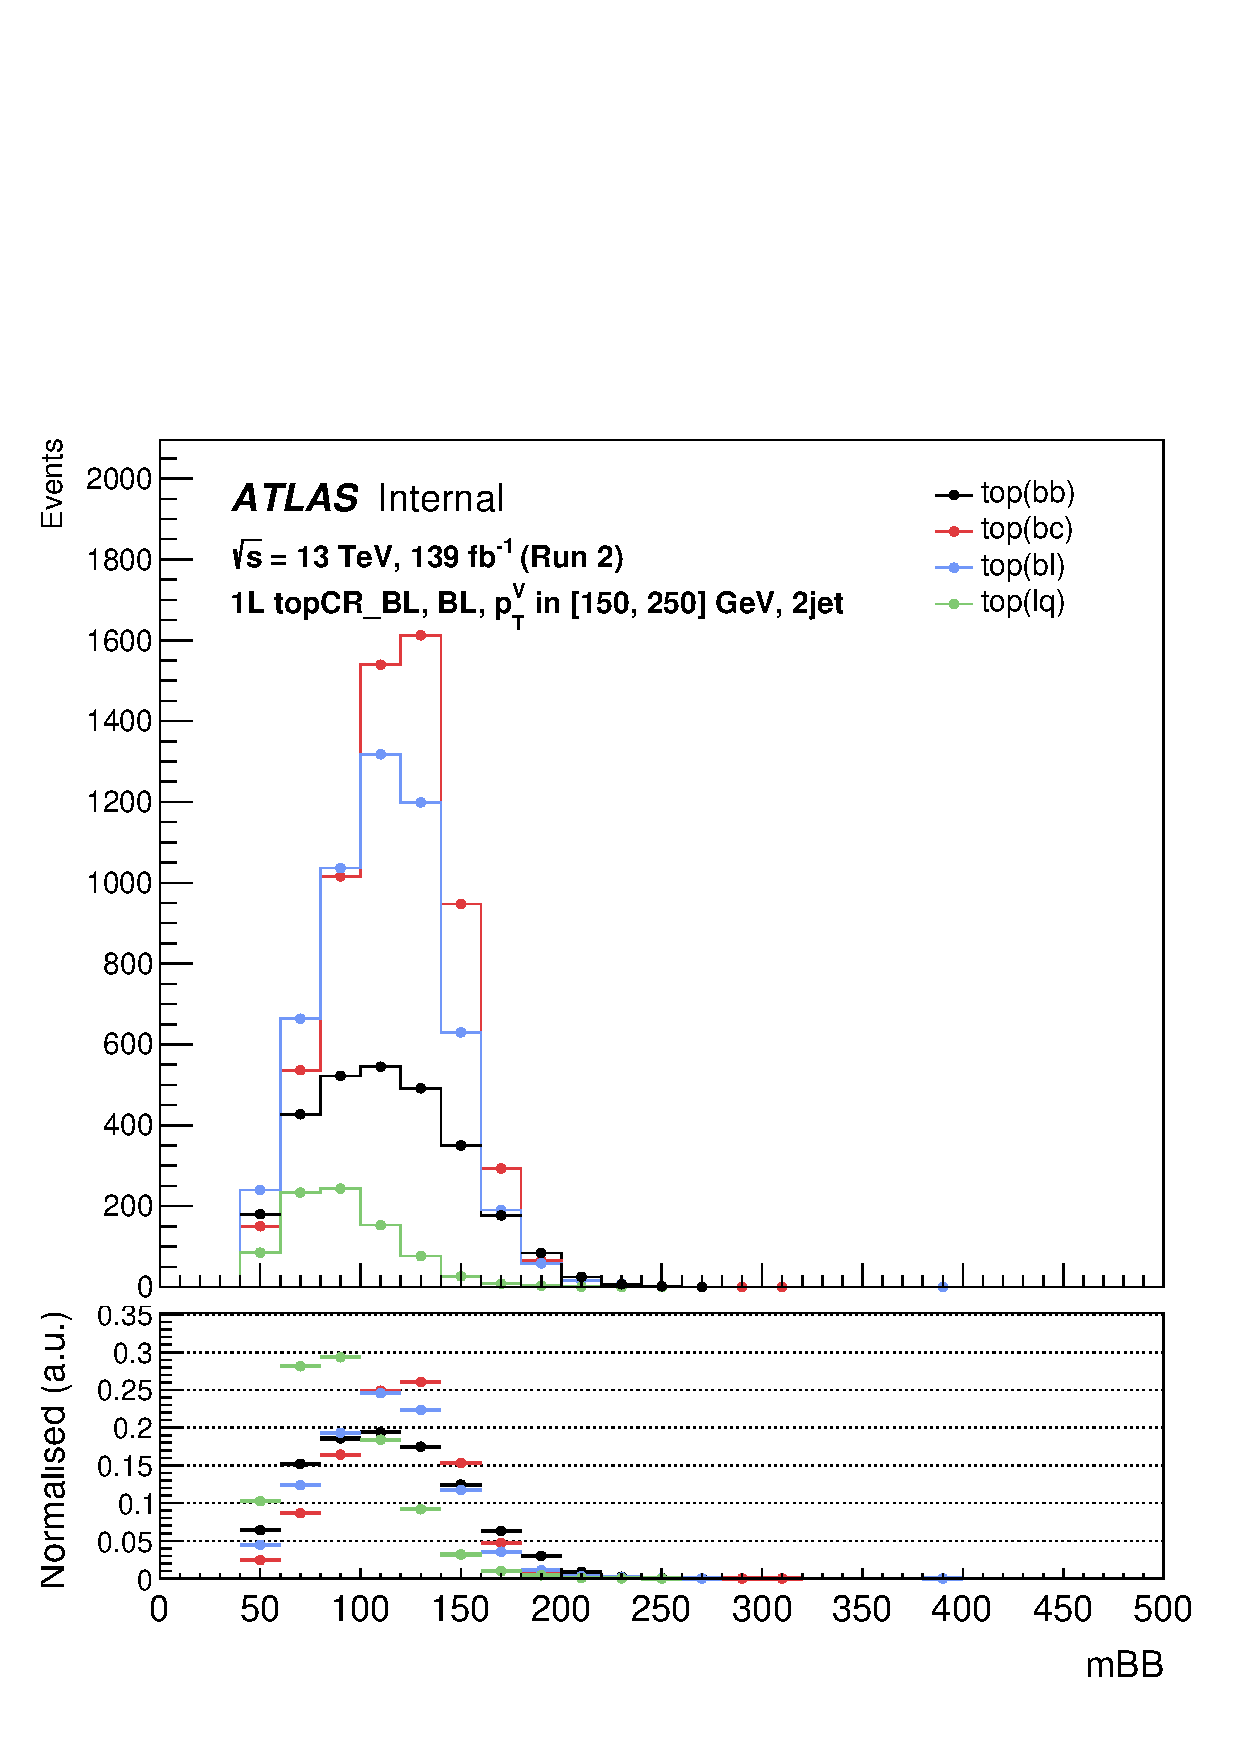
\includegraphics[scale=0.253]{Images/VH/top/OneLepton_top_1bltag2jet_topCR_BL_150_250ptv_mBB.pdf}
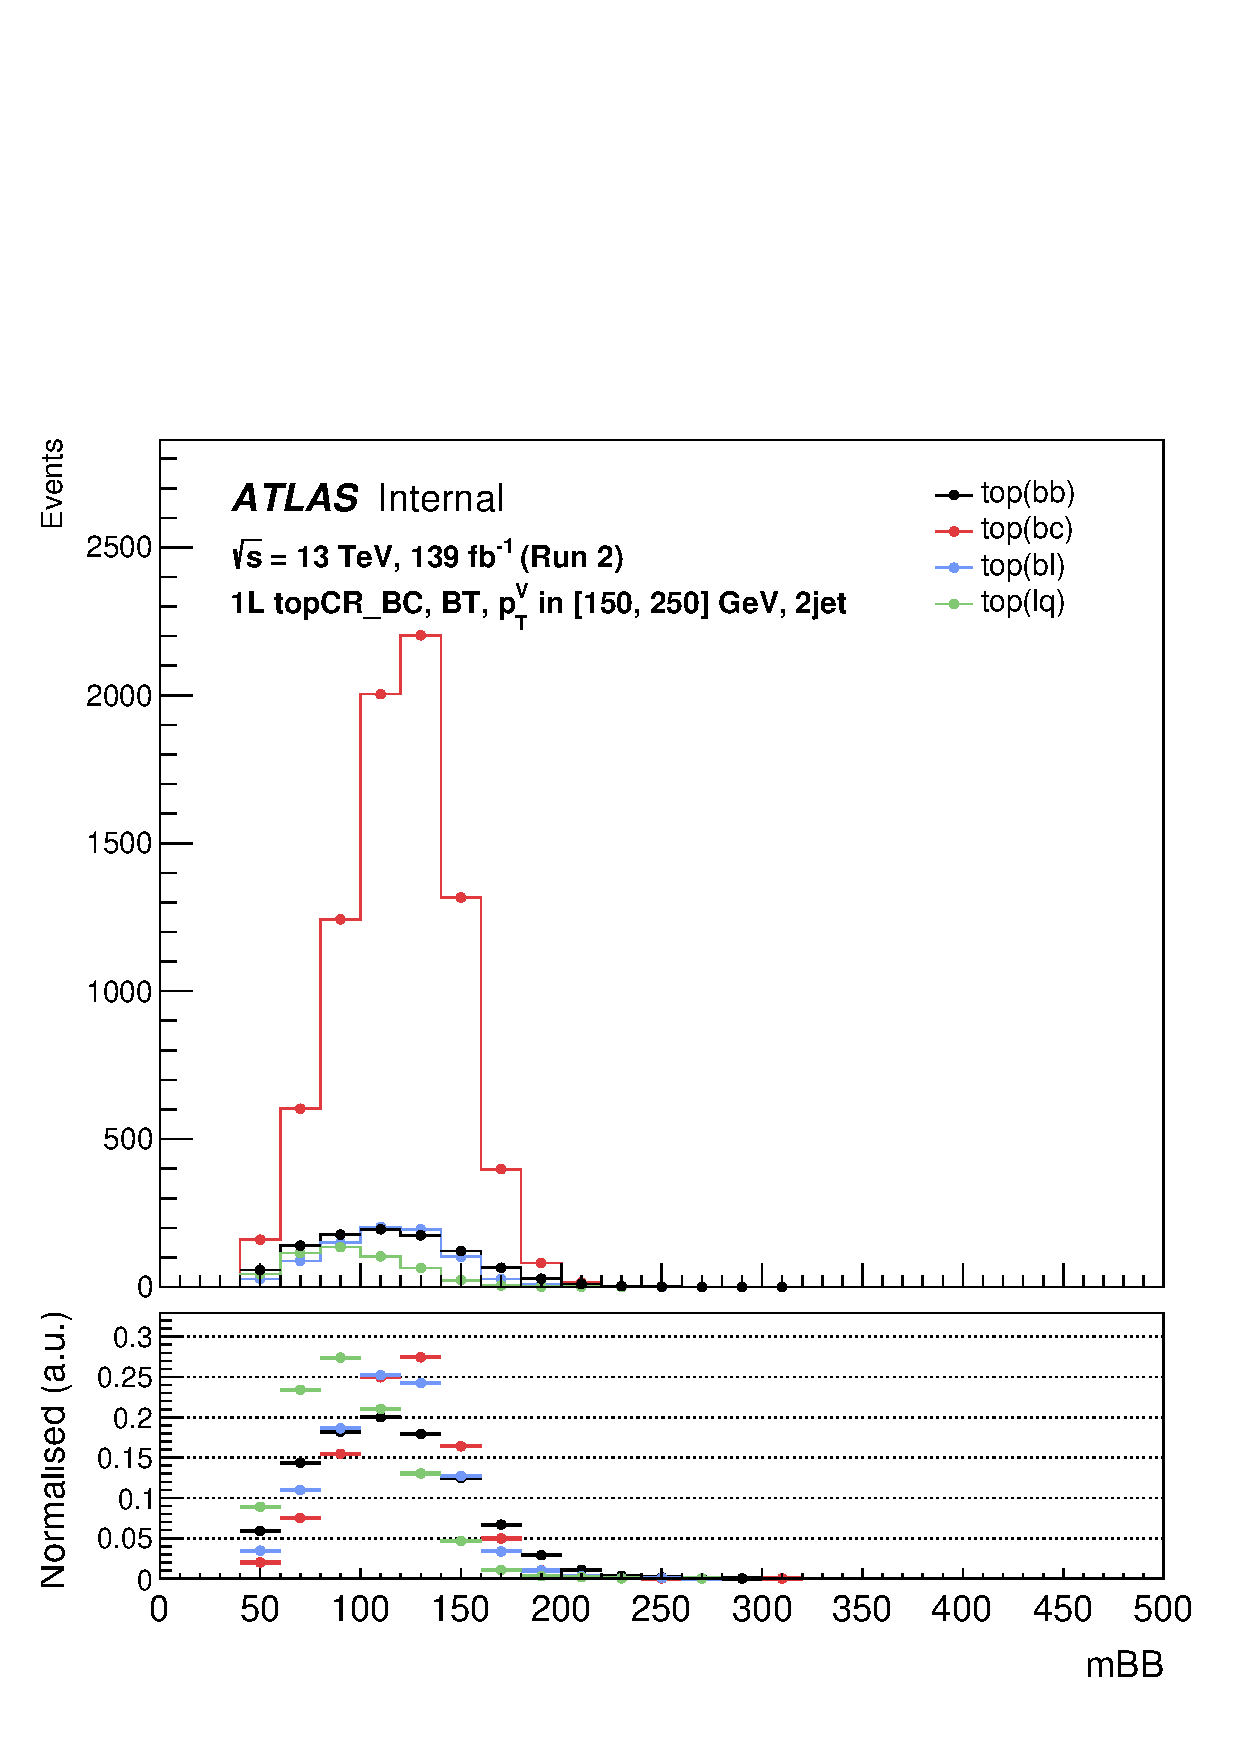
\includegraphics[scale=0.253]{Images/VH/top/OneLepton_top_1bttag2jet_topCR_BC_150_250ptv_mBB.pdf}\\
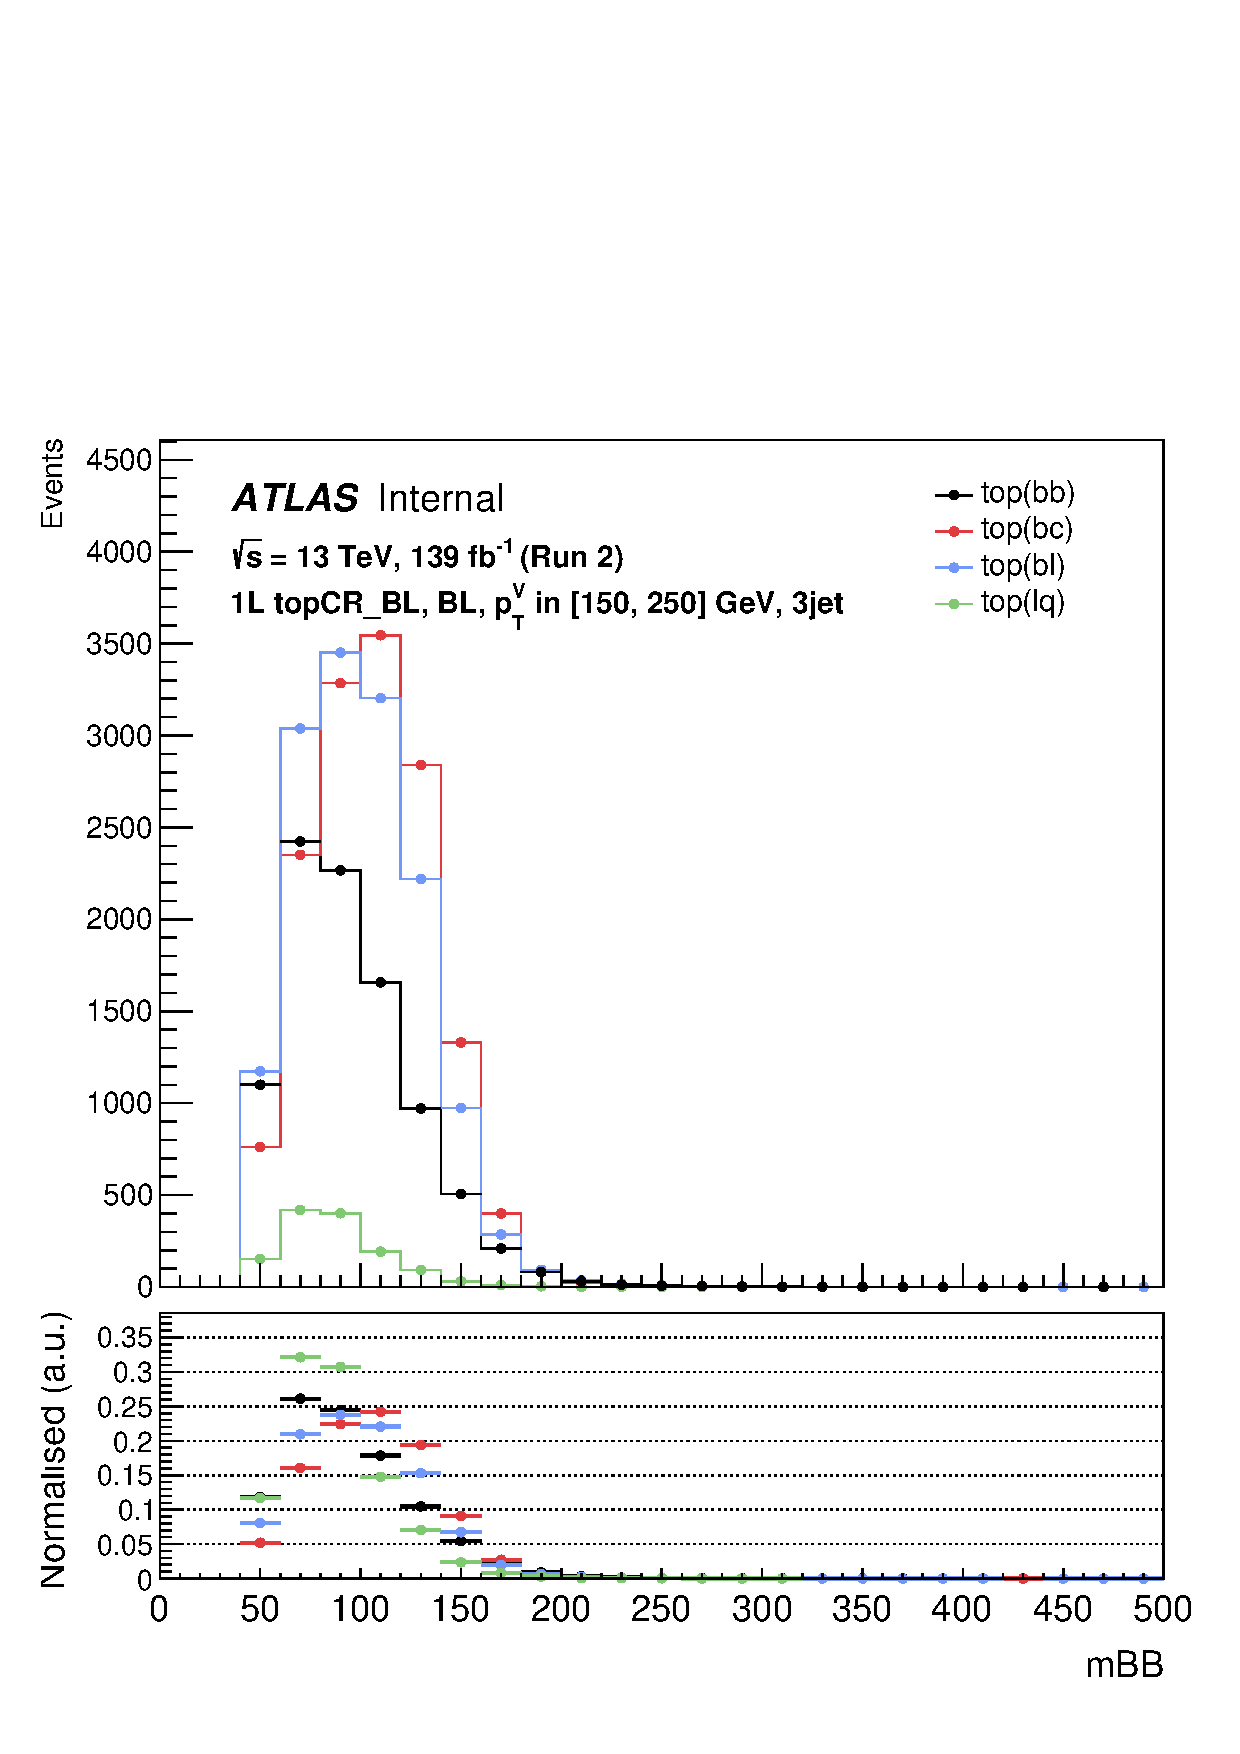
\includegraphics[scale=0.253]{Images/VH/top/OneLepton_top_1bltag3jet_topCR_BL_150_250ptv_mBB.pdf}
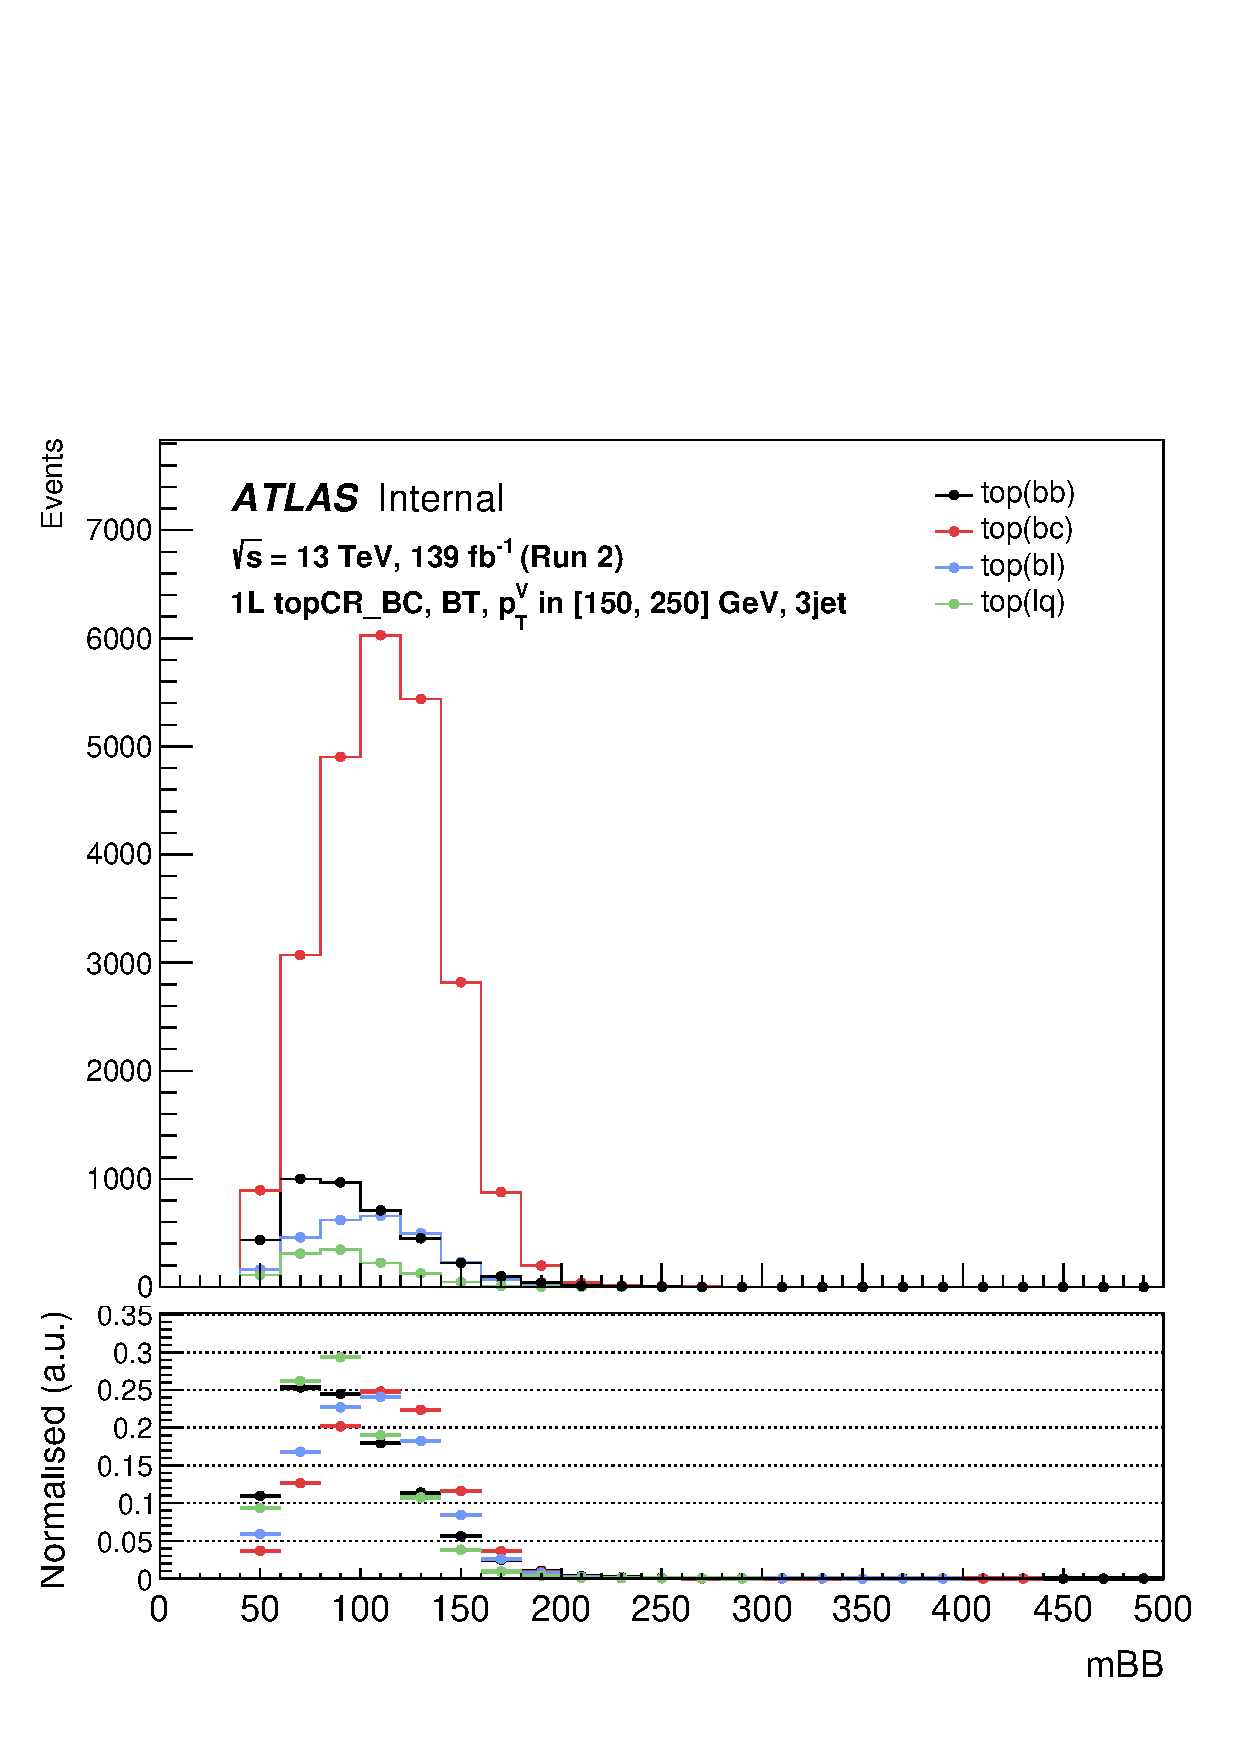
\includegraphics[scale=0.253]{Images/VH/top/OneLepton_top_1bttag3jet_topCR_BC_150_250ptv_mBB.pdf}
\caption{The top components in the 1L top CR regions ($m_{c\bar{c}}$ distributions) in the low [150-250] $p_T^V$ range. Left: BL region; right: BT region. Top: 2 jets, bottom: 3 jets.} 
\label{fig:toptopCRslowptv}
\end{figure}

\begin{figure}[h!]
%\hspace{-2.0cm}
\center
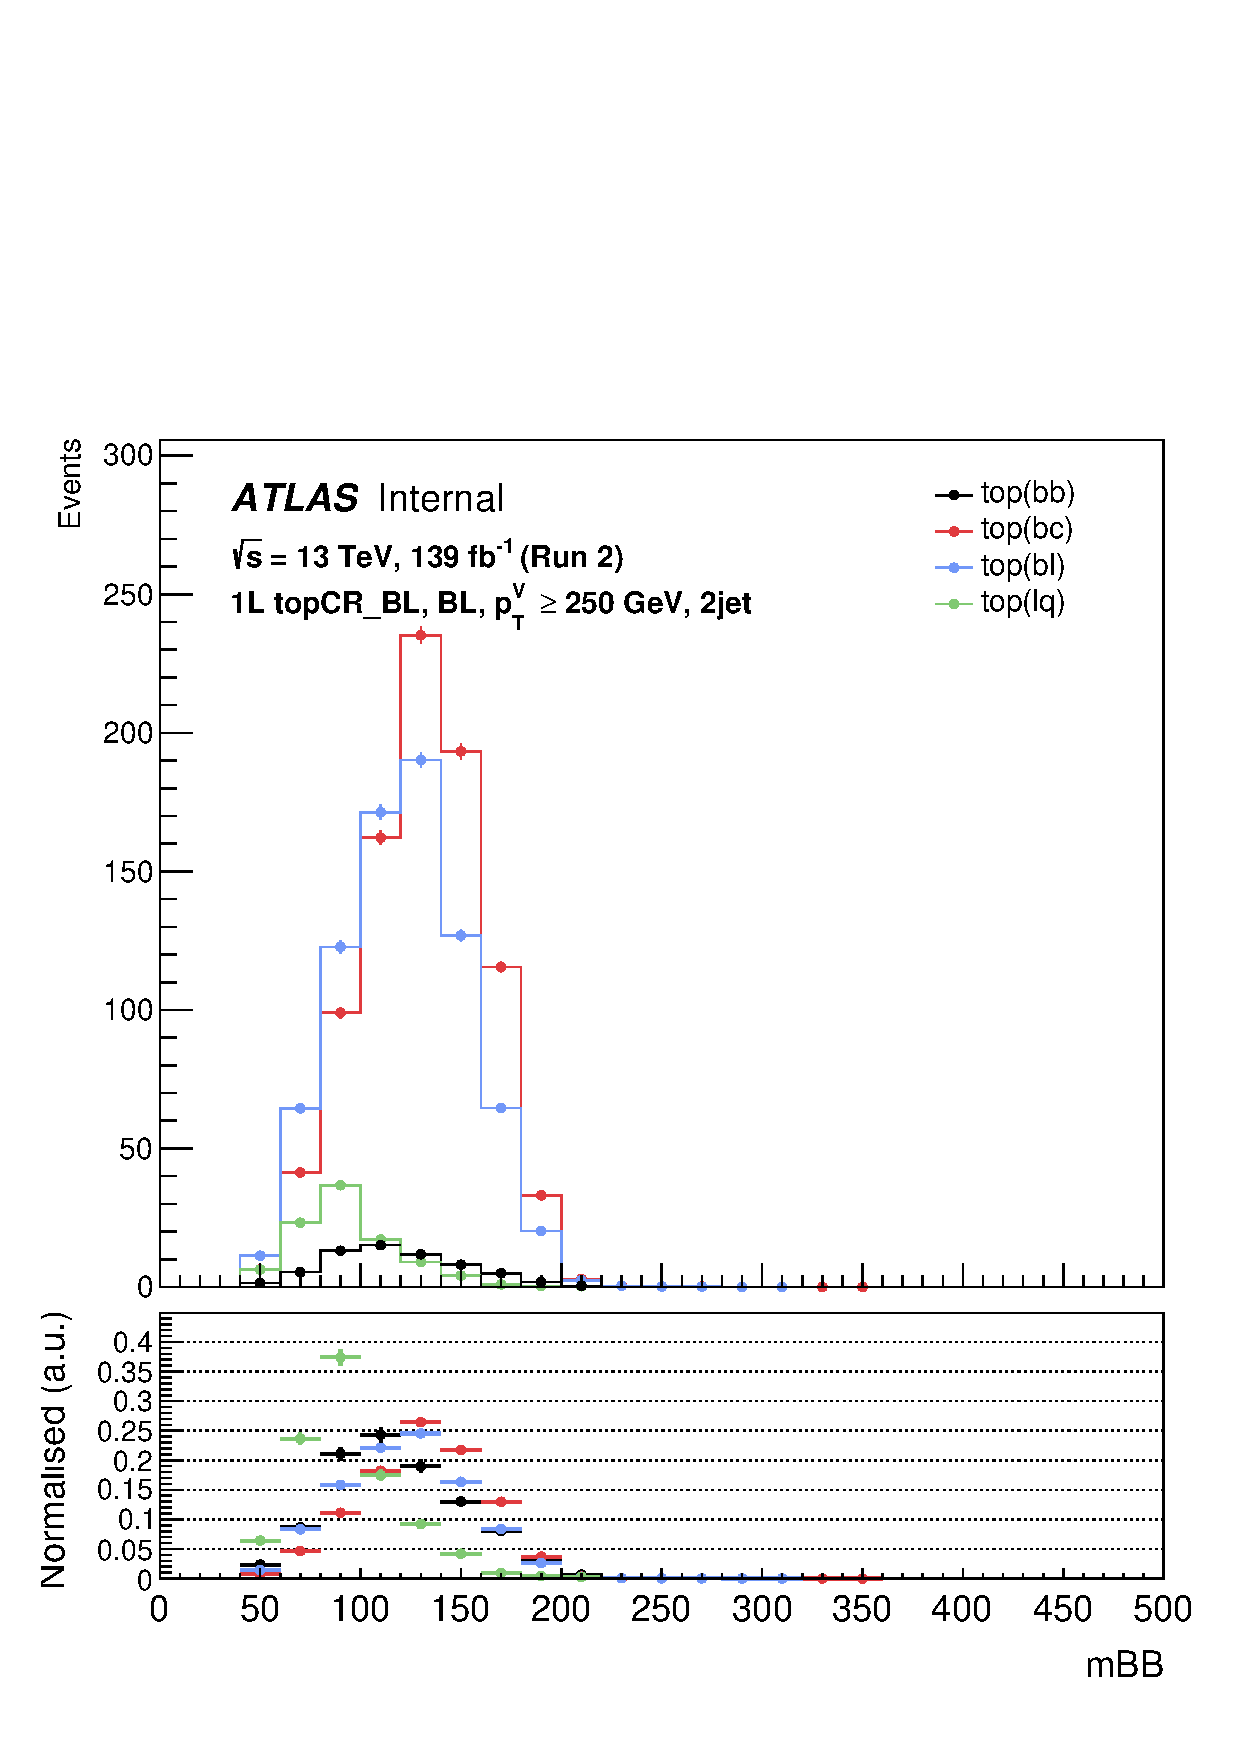
\includegraphics[scale=0.253]{Images/VH/top/OneLepton_top_1bltag2jet_topCR_BL_250ptv_mBB.pdf}
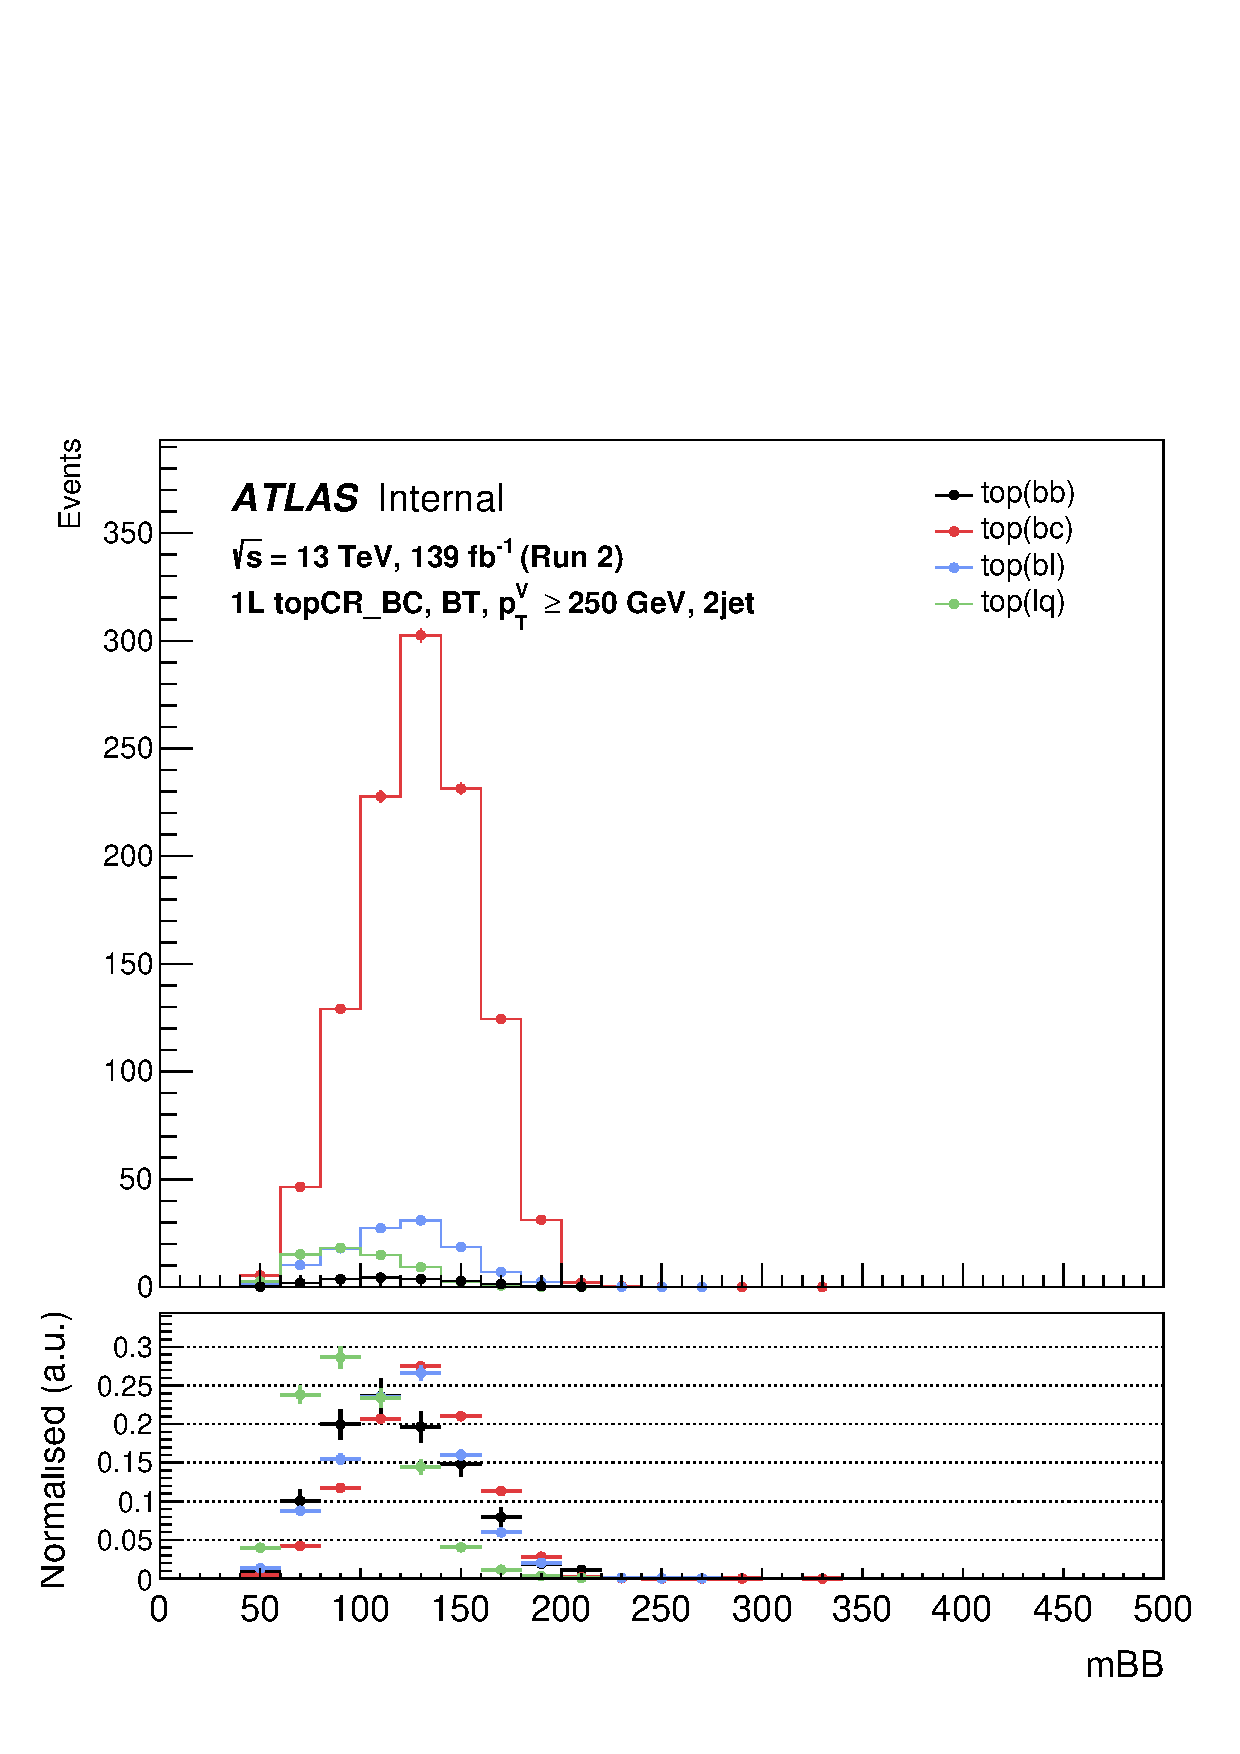
\includegraphics[scale=0.253]{Images/VH/top/OneLepton_top_1bttag2jet_topCR_BC_250ptv_mBB.pdf}\\
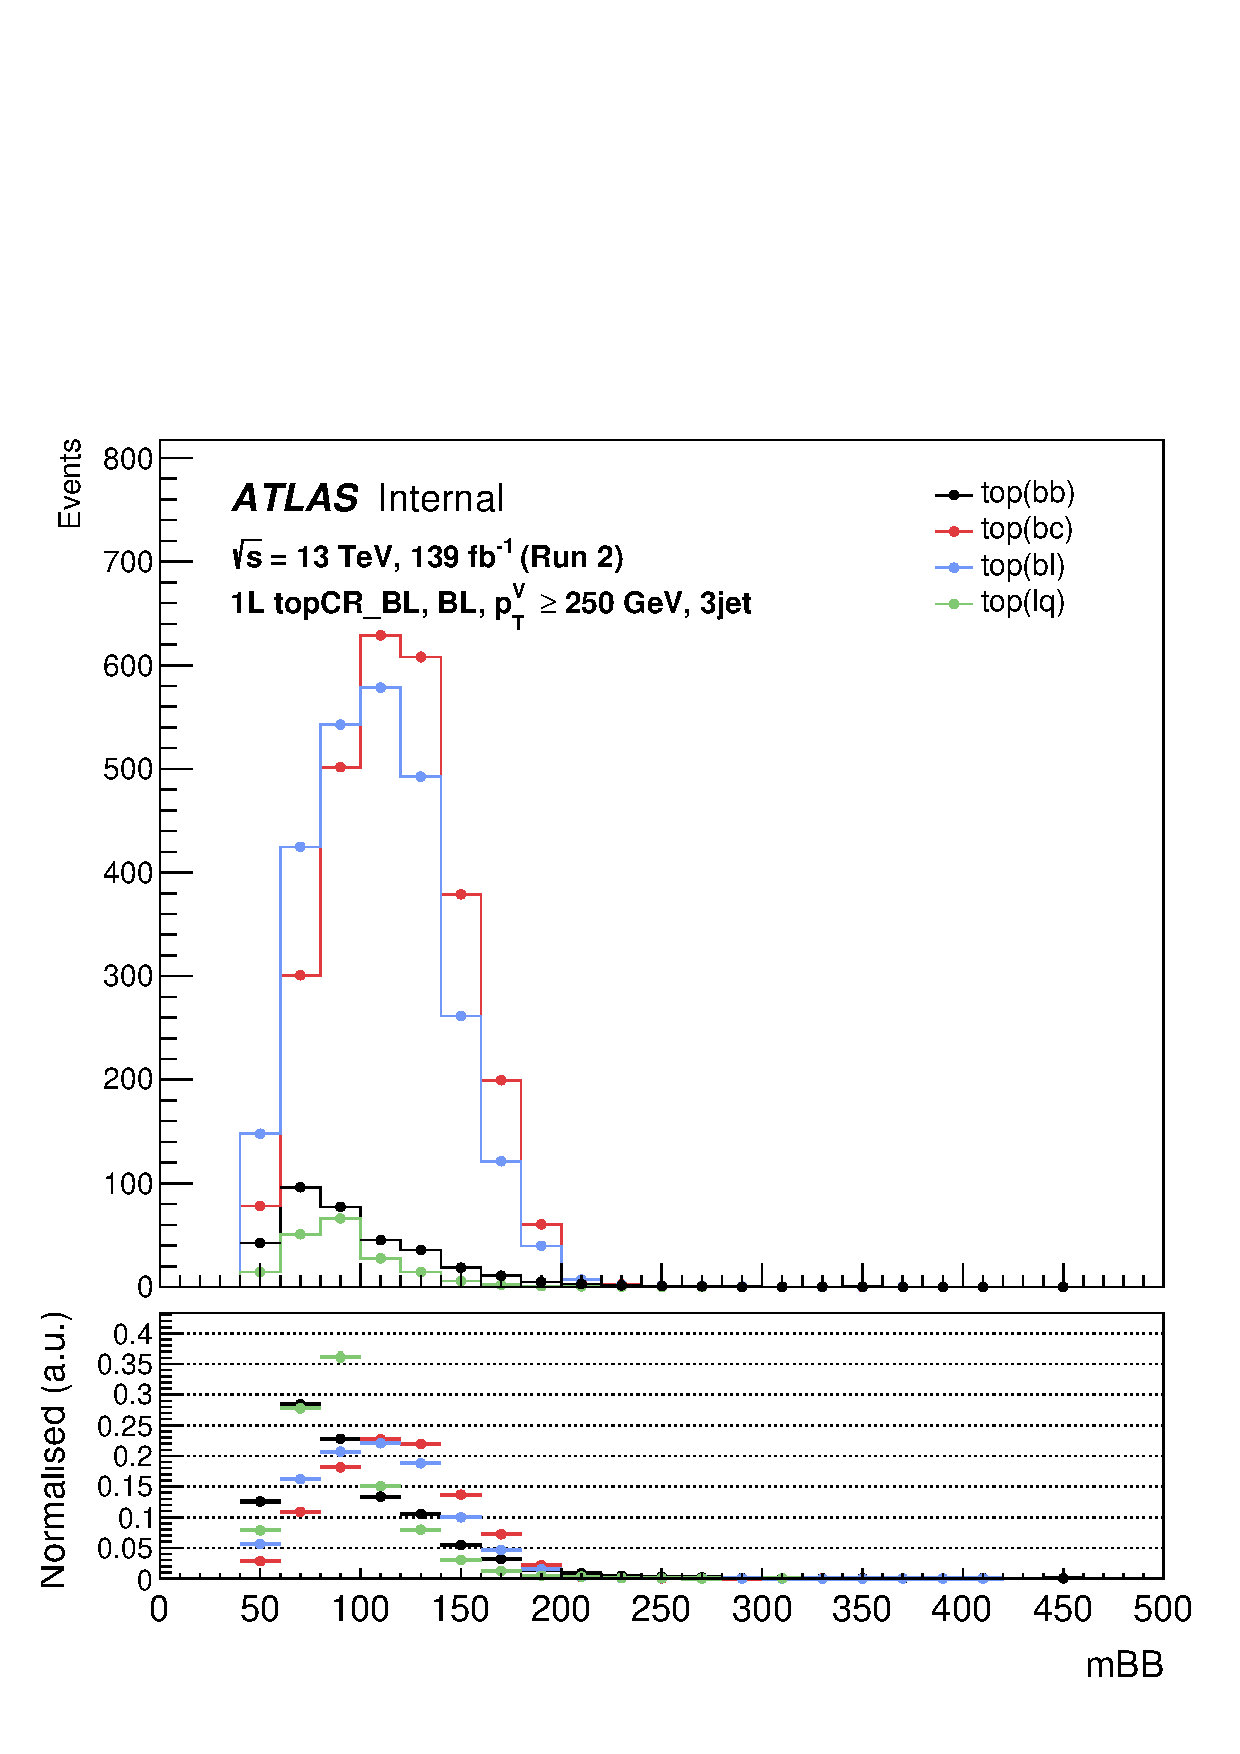
\includegraphics[scale=0.253]{Images/VH/top/OneLepton_top_1bltag3jet_topCR_BL_250ptv_mBB.pdf}
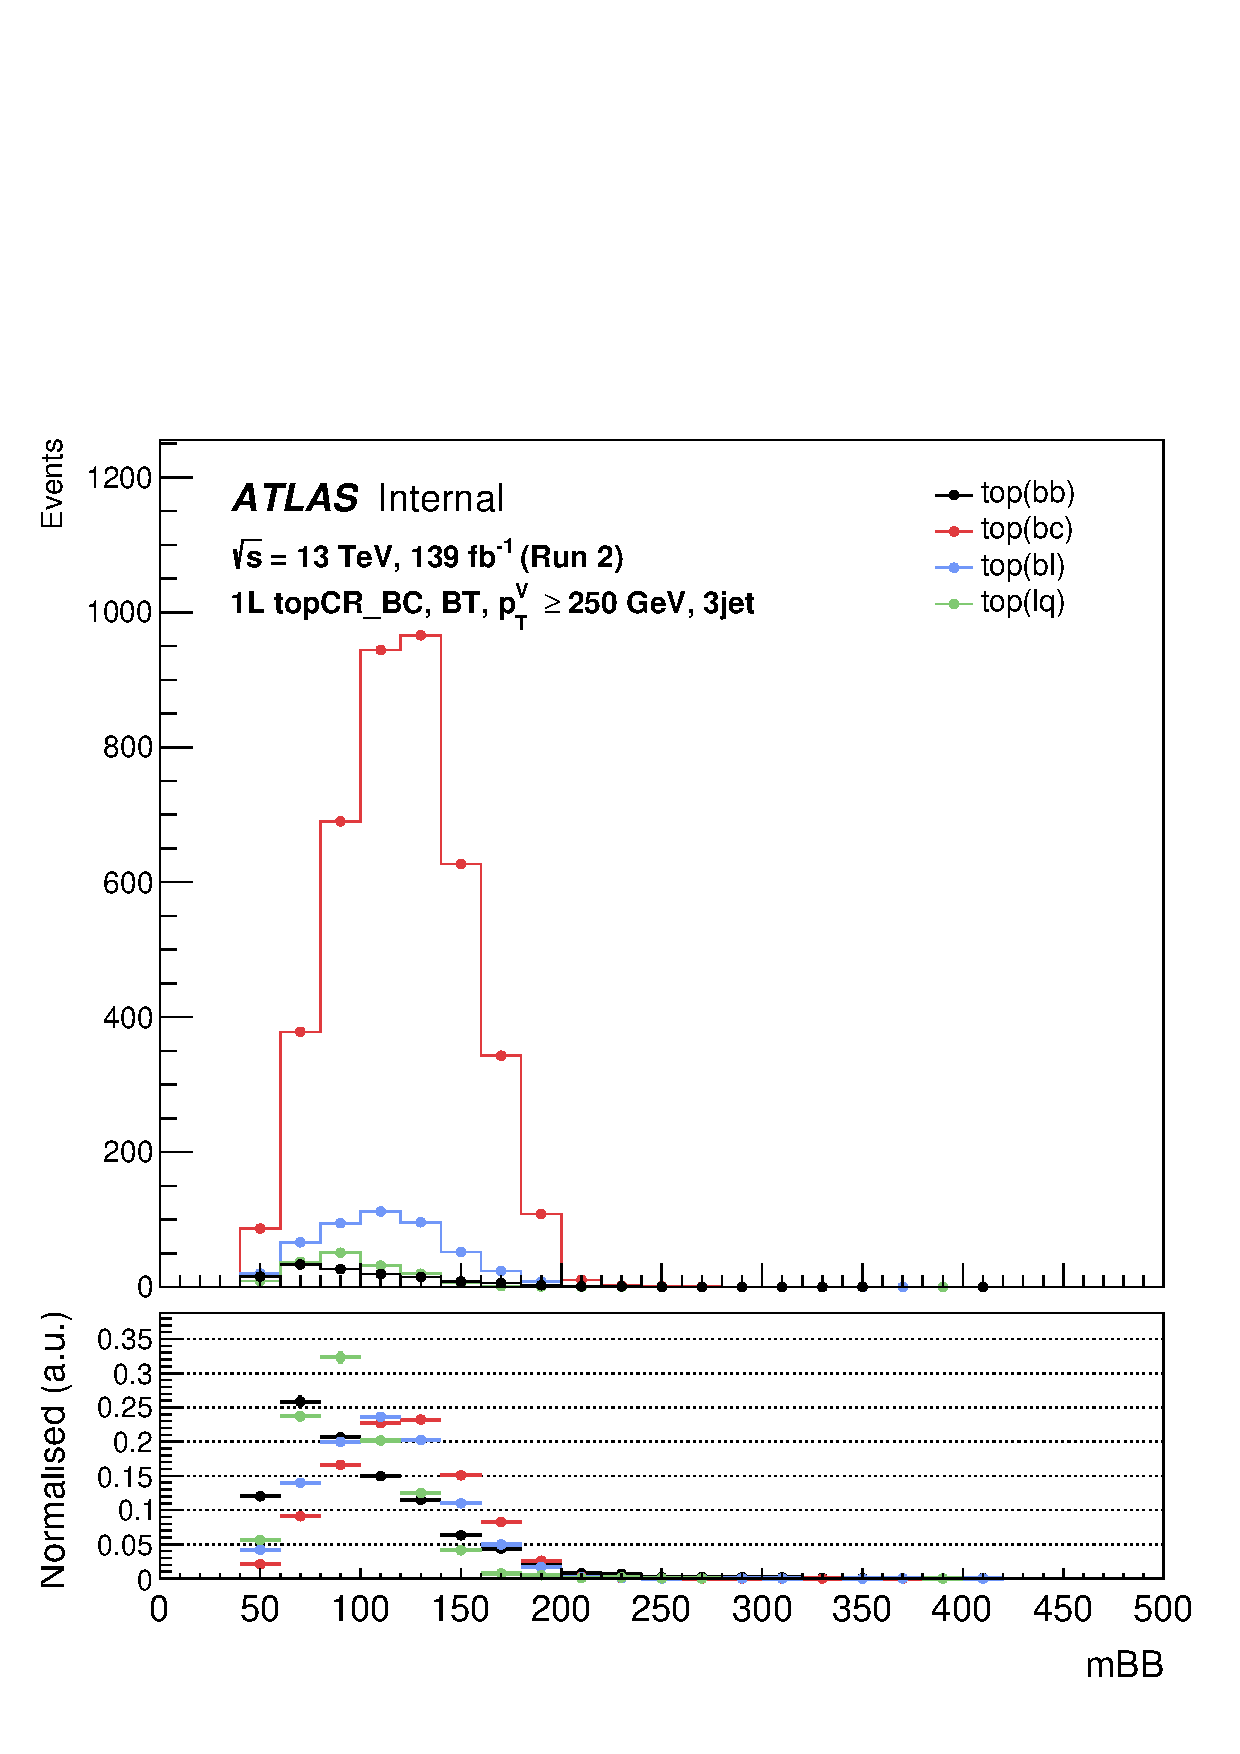
\includegraphics[scale=0.253]{Images/VH/top/OneLepton_top_1bttag3jet_topCR_BC_250ptv_mBB.pdf}
\caption{The top components in the 1L top CR regions ($m_{c\bar{c}}$ distributions) in the high  > 250 $p_T^V$ range. Left: BL region; right: BT region. Top: 2 jets, bottom: 3 jets.} 
\label{fig:toptopCRshighptv}
\end{figure}
